%!TEX TS-program = pdflatex
%!TEX root = i3det-top.tex
%!TEX encoding = UTF-8 Unicode

% additional definitions
\newcommand{\degC}[1]{$\unit[#1]{^\circ{C}}$}
%\newcommand{\mA}{\mbox{\unit{mA}}}
% definition to produce a "less than or similar to" symbol
\def\lsim{\mathrel{\rlap{\raise 0.2ex\hbox{$\,<\,$}}{\lower 0.9ex\hbox{$\,\sim\,$}}}}
% definition to produce a "greater than or similar to" symbol
\def\gsim{\mathrel{\rlap{\raise 0.2ex\hbox{$\,>\,$}}{\lower 0.9ex\hbox{$\,\sim\,$}}}}


\section{The Digital Optical Module}
\textsl{(Chris Wendt; 10 pages)}

\subsection{\label{sec:dom_functional} A Functional Description of the DOM}

The DOM is the fundamental light sensor and data acquisition unit for IceCube.
It consists of a spherical glass housing 
containing a downward-facing $10^{\prime\prime}$ diameter photomultiplier tube (PMT)
and associated circuit boards that allow near-autonomous operation (Figure~\ref{fig:domcomponents}) .
Data acquisition, control, calibration, communication and low voltage power conversion 
are integrated in one annular circuit board that fits around the neck of the PMT (Main Board)~\cite{ref:domdaq}. 
Separate circuit boards generate PMT high voltage, interface to the PMT pins~\cite{ref:pmt},
delay PMT signals, and generate calibration light flashes that can reach other DOMs.
Key requirements for the DOM include
the precise recording of a wide variety of PMT pulse widths and amplitudes, robustness in
a challenging deployment environment, and long term reliability.

%============================================================
\begin{figure}
\vspace{3pt}
\begin{center}
\begin{tabular}{c@{\hspace{0pt}}c}
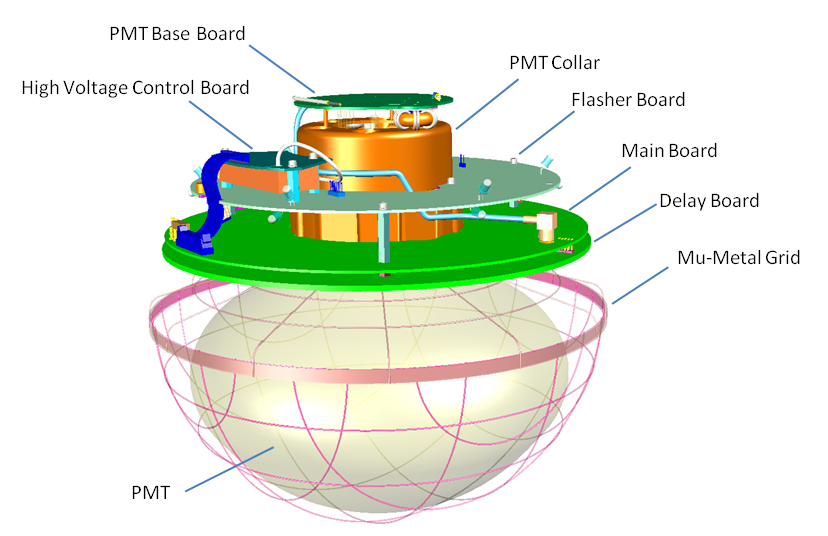
\includegraphics[width=0.49\textwidth,clip=true]{graphics/dom/functional/domfig1a-DOM3DModel.png} & \
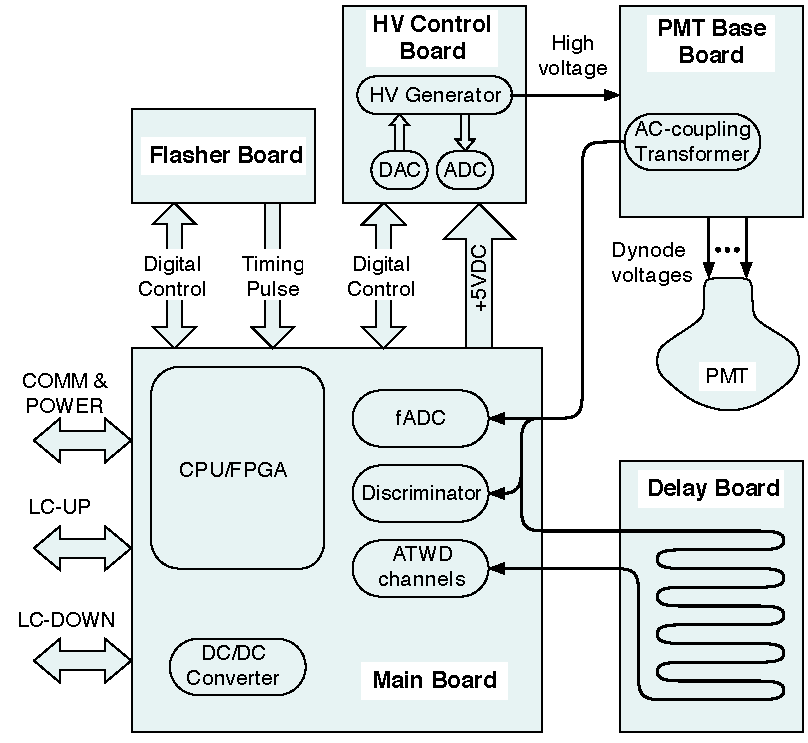
\includegraphics[width=0.49\textwidth,clip=true]{graphics/dom/functional/domfig1b-DOMBlockDiagram.pdf} \\
\end{tabular}
\end{center}
\caption{Components of the DOM, showing mechanical layout (left) and functional connections (right).
}
\label{fig:domcomponents}
\end{figure}
%============================================================


The PMT detects
signals from neutrino events ranging over energies \unit[10]GeV--\unit[10]PeV
and  distances  from a few meters to \unit[500]m away.
Corresponding PMT waveforms can have amplitudes from \unit[1]mV up to and beyond the linearity limit
of the PMT (\unit[$\sim2$]volts) and widths from \unit[12]nsec to \unit[1500]nsec.
In order to accommodate such a variety of signals,
the DOM includes multiple digitizers with overlapping dynamic range and different sampling speeds
(Section~\ref{sec:mainboard})~\cite{ref:domdaq}.
Each DOM is triggered independently by detection of individual photons, starting a 
recording of the PMT waveform that includes further photons arriving up to \unit[6.4]{$\mu$sec} later.
The trigger time is saved along with the
waveform shape, which reveals the times of arriving photons relative to this reference.
The DOM typically accumulates such triggered data for a period of ? to \unit[?]sec before sending as a block.
Separately, the PMT trigger rate is recorded in \unit[0.1]sec intervals,
as a collective increase of all rates could signify detection of many low energy neutrinos
in case of a galactic supernova event~\cite{ref:supernova}.

DOMs transmit their data to computers in the IceCube Laboratory building using a twisted wire pair that also provides
power.  Wire pairs are bundled together to form the vertical down-hole cables and the horizontal surface cables.  
Each wire pair is shared between two DOMs, with data transfers initiated by a surface computer.
Separately, dedicated wiring to neighbor DOMs above and below allows 
quick recognition of local coincidences where nearest or next-to-nearest neighbors trigger within
a common \unit[1]$\mu$sec time window.
Local coincidence triggers often have complex PMT waveforms reflecting multiple photons
detected in each DOM, which are therefore
saved in full detail; otherwise the DOM saves abbreviated information appropriate to single photon
detection (Section~\ref{sec:mainboard})~\cite{ref:domdaq}.

The DOM is capable of interpreting commands from the surface that specify tasks for configuration, 
data taking and transmission, monitoring or self-calibration.
Self-calibration functions establish PMT and amplifier gains as well as sampling speed (Section~\ref{sec:domcal}).
The RAPCal system(Section~\ref{sect:dom:rapcal}) is implemented for tracking each local DOM clock's offset from universal time,
allowing PMT pulses that were independently recorded in many DOMs  to be recombined into events by surface computers.

\subsection{\label{sec:dom_components} Components}

\subsubsection{\label{sec:sphere}Glass Sphere and Harness}

The glass sphere housing has diameter $13^{\prime\prime}$ and thickness $0.5^{\prime\prime}$.  
Spheres are specified to protect the inside electronics and PMT against long term applied pressure of 
\unit[250]bar (\unit[2.6]km water depth)
as well as temporary overpressure up to \unit[690]bar during refreezing of melted ice in the drill hole.
They were produced by Benthos, Inc., based on a design for deep sea environments but using glass
with very low potassium or other radioactive trace elements that would contribute to the dark noise
count rate (Section~\ref{sect:darknoise}).  
%N.B. not borosilicate, according to analysis shown at final CDR 2005 (Claire's slides), in contrast
%to the Benthos sphere datasheet which says borosilicate
Optical transmission was measured in representative samples as 93\% at \unit[400]nm,
decreasing to 50\% at \unit[340]nm and 10\% at \unit[315]nm (normal incidence, excluding Fresnel reflection).

All spheres were tested up to \unit[10,000]psi hydrostatic pressure by the manufacturer.
Each was delivered as two hemispheres that mate precisely at the equator.
After assembly of other components into the sphere, it is evacuated and backfilled with dry nitrogen,
a butyl rubber sealant is applied around the seam, and the sealant is covered with wide plastic tape.
The interior gas pressure is set to 0.5 bar so the seal remains tight even
at ambient south pole air pressure 0.6 bar.

The DOM is held by an aluminum waistband with rubber gaskets against
the glass above and below the equator seam. 
Figure~\ref{fig:domcable} shows how it is attached to the main down-hole cable via a system
of steel rope and chain that carries the weight load around the DOM.
The main cable bends around the DOM, and the DOM axis stays vertically aligned with the string.

%============================================================
\begin{figure}
\vspace{3pt}
\centering
\begin{tabular}{c@{\hspace{0.5in}}c}
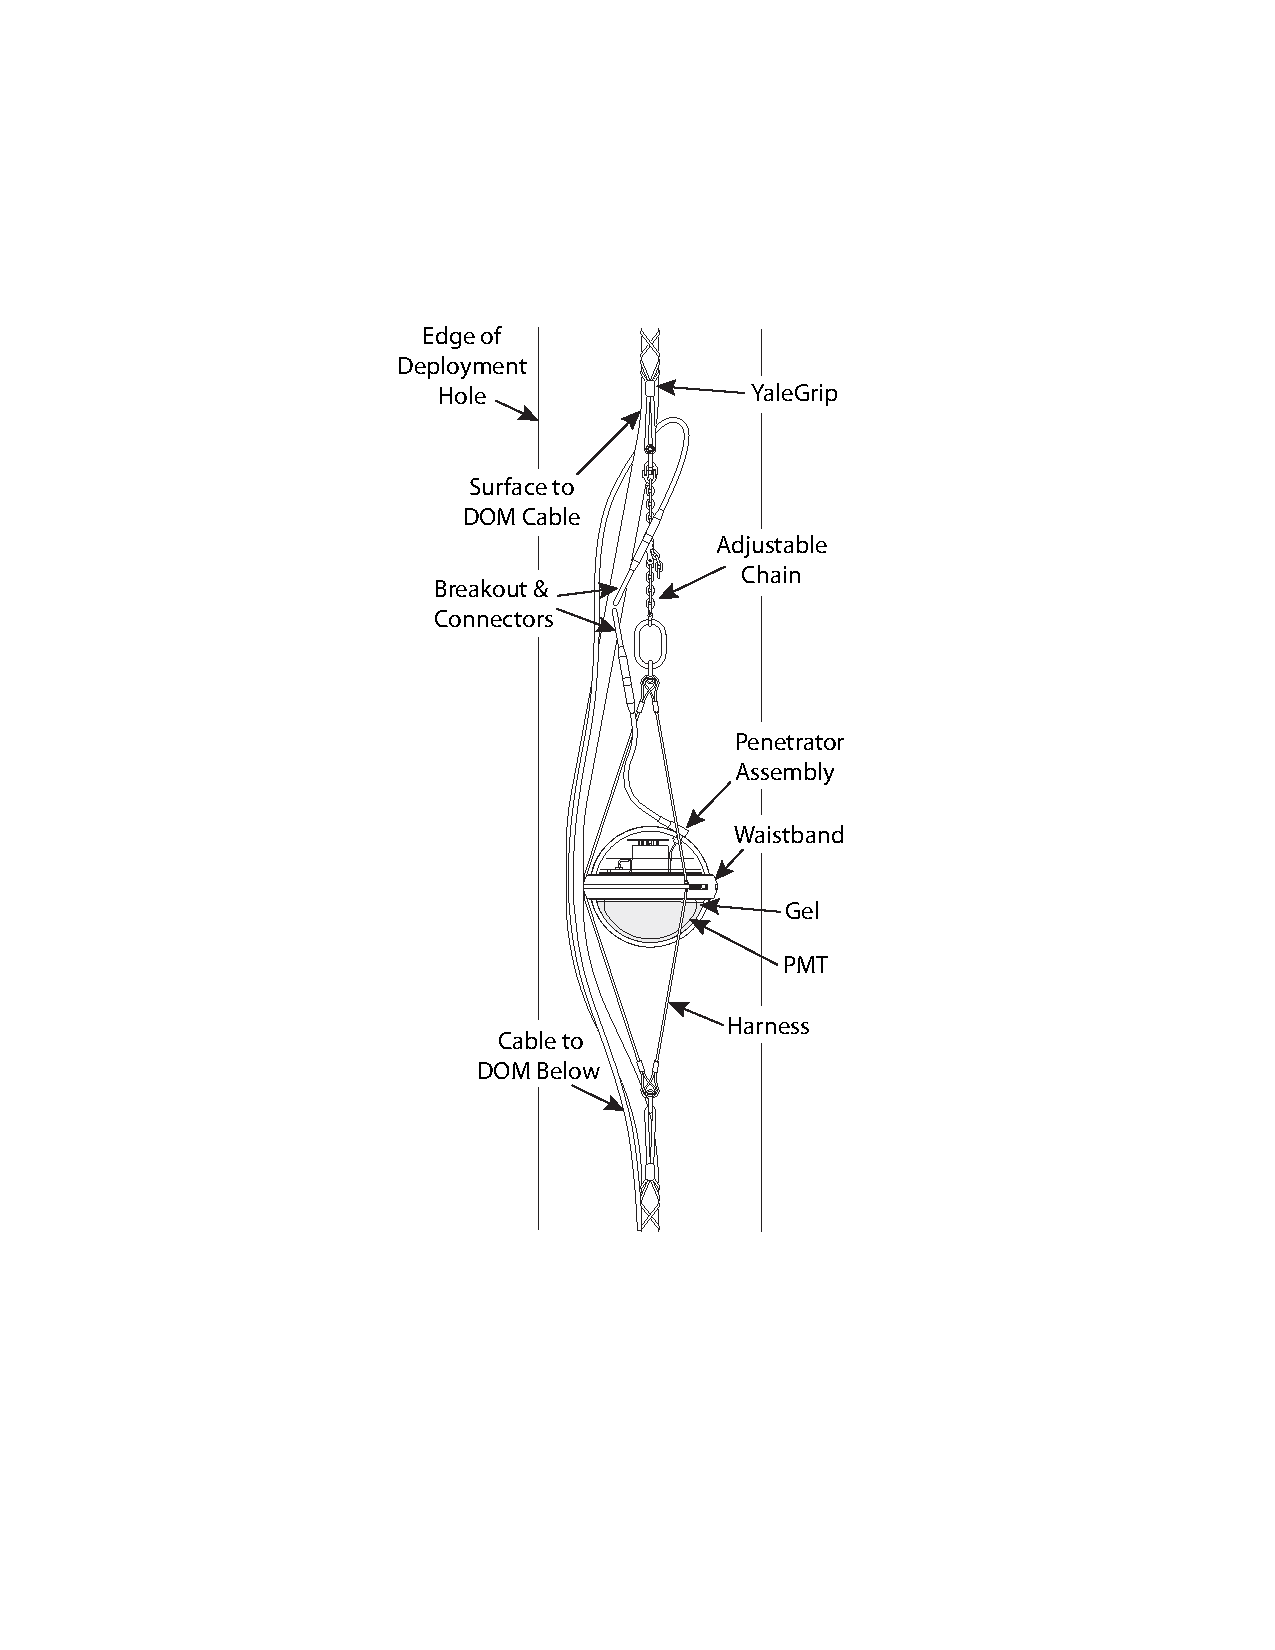
\includegraphics[width=0.3\textwidth,clip=true]{graphics/dom/functional/domfig2a-CableAssembly.pdf} & \
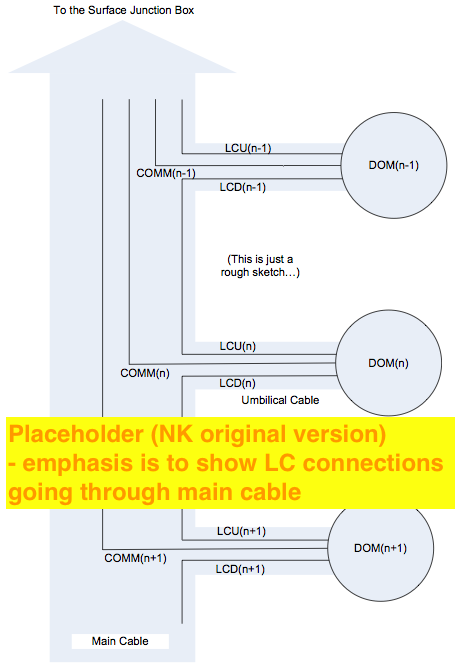
\includegraphics[width=0.4\textwidth,clip=true]{graphics/dom/functional/domfig2b-CableConnections.png} \\
\end{tabular}
\caption{FIXME Figure to be updated. 
(Left) DOM as deployed on main downhole cable, showing cable breakout to the penetrator
assembly and the mechanical support system.  (Right) Schematic of cable connections, 
illustrating the sharing of each communications wire
pair by two DOMs and the additional wire pairs used for local coincidence signaling between
neighboring DOMs.
}
\label{fig:domcable}
\end{figure}
%============================================================

%NK section 3.4.1 text:
%The spherical pressure housing consists of two hemespheres made of low expansion borosilicate
%glass that seal at the equator. Each pair of mating hemespheres have been tested for pressure
%tightness at 10,000 psi (689 bar) by the manufacturer. [The pressure must operate continuously
%under 250 bar (2.6 km-deep water) and allow the over pressure of 689 bar (refreezing pressure) for
%seven days. 9400-0029-PCR.] The top hemesphere has a 16.3 mm-diameter hole for installing the
%penetrator assembly (below) that facilitates electrical connections to the interior electronics without
%compromising the pressure tightness.
%The pair of glass hemespheres consitutes more than 9 Kg of mass (9.07 Kg) and is potentially a
%significant source of photonic noise arising from the decay of radioisotope content. The IceCube
%spheres are produced with a special attention to eliminate pottasium content and minimize other
%radioactive trace elements, such as cerium. [According to Chemir Analytical Services report, June
%2005, the pottasium concentration was below the detection level and that of cerium was less than
%40 ppm by ICP analysis; however, in a separate University of Washington measurement, non-zero
%numbers are seen under pottasium. Without any write up to accompany the measurement, we
%don’t know how to interpret the numbers.] The manufacturer’s standard material contains CaCO3
%(calcite), known to have fluorescent properties, which was also eliminated [Presumably. See Kael’s
%report, November 2003]. 

\subsubsection{\label{sec:penetrator}Cable Penetrator, Cable and Connector}

%NK section 3.4.2 text:
%(This includes the external umbilical, the internal pigtail, and the connectors on either end.) Each
%DOM requires three wire-pair connections to its interior: one pair is connected to the surface DAQ
%system and carries the bidirectional communication signals and power; another two pairs provide
%local coincidence connections to the neighboring DOMs, one above and one below.
%The penetrator is an assembly of cables and electrical feedthrough that accomplishes the 
%necessary electrical connections from outside the pressure housing through its wall while maintaining the
%pressure-tightness, characteristic impedance, and signal cross-talk requirements. It consists of a
%threaded stainless steel feedthrough that achieves the pressure-tightness by means of a single
%o-ring pressed against the glass exterior and is tightened with a spring washer and a locking nut
%from inside; a pig-tail cable that connects to the DOM main board; and a custom-designed umbili-
%cal cable containing three shielded twisted-pair cables within its jacket and having a pressure-tight
%multi-pin connector that plugs into the mating connector at one of the breakouts (see below) of the
%main cable. The umbilical cable is 0.7 m long for the type U DOM and 19.2 m long for the type T
%DOM. The umbilical cable is terminated with a dissimilar connector depending on the type of the
%DOM in order to avoid a wrong connection by human error during the deployment.

A penetrator assembly brings three wire pairs out through a \unit[16.3]mm hole in
the DOM glass.  They are routed inside a customized cable, visible in Figure~\ref{fig:domcable},
and terminate at a pressure-tight, waterproof connector that mates with a similar connector
that continues each pair into the main cable.  One wire pair carries power and a
bidirectional digital communications stream, connecting ultimately with computers in the
IceCube Laboratory building (Section~\ref{sec:cablesystems}).
The other wires lead to neighbor DOMs directly above and below,
carrying local coincidence digital pulses that signify time correlated hits in nearby DOMs (Section~\ref{sec:mainboard}).

DOMs were made in two versions, where the communications wire pair was either electrically
terminated (\unit[150]$\Omega$) or unterminated inside the DOM.  This allows each wire pair from
the surface computers to communicate with two DOMs in parallel; the terminated one is deployed
\unit[17]m below the unterminated one (\unit[7]m or \unit[10]m in DeepCore strings) and therefore includes a correspondingly
long penetrator assembly cable (bottom of Figure~\ref{fig:domcable}).

The entire penetrator assembly was custom designed and produced by SEACON (California).  The part that seals against
the DOM glass is similar to a hollow steel bolt, which is secured inside the DOM by a nut and spring washer and compresses
a fluorosilicone o-ring against the outside surface.  The steel part includes additional sealing around the wires that pass through it.
Outside the DOM, a plastic shell is molded around the steel and onto the cable jacket.  
External mechanical features like the penetrator are subject to large stresses during deployment and the refreezing process;
a right angle bend outside the DOM was included for robustness, based on previous experience deploying AMANDA modules.


\subsubsection{\label{sec:pmt}PMT, Gel and Magnetic Shield}

%NK text: The gel’s primary purpose is optical coupling between the sphere and the PMT; 
%however, it also serves as a mechanical shock absorber to protect
%the PMT and the electronic assemblies during the handling, transport, and deployment. All other
%components are mounted on the PMT and no components make a mechanical contact with the
%pressure housing wall, except for the pigtail cable of the penetrator.

DOMs use the $10^{\prime\prime}$ diameter Hamamatsu R7081-02 PMT, 
or the corresponding high-quantum-efficiency (HQE) version for Deep Core strings.
Its properties have been measured and described in \cite{ref:pmt}.  It is specified by Hamamatsu for
the wavelength range \unit[300]nm--\unit[650]nm, with peak quantum efficiency around 25\% (34\% for HQE)
near \unit[390]nm.  It features a box-and-line dynode chain with 10 stages, and is operated at gain $10^7$
(Section~\ref{sec:domcal}).

The PMT bulb faces downwards in the bottom glass hemisphere, secured in high-strength 
silicone gel to a depth surrounding the photocathode area.  
The gel provides mechanical support for the whole assembly of PMT and circuit boards,
as well as good optical coupling.  
Gel thickness between PMT envelope and glass sphere is approximately \unit[1]cm.  
Originally the gel was supplied as General Electric RTV6136-D1,
and later as a similar formulation from Quantum Silicones (Virginia, USA).  
It is optically clear with transmission 97\% at \unit[400]nm, 91\% at \unit[340]nm, and 65\% at \unit[300]nm
(normal incidence).  The refractive index is 1.41, yielding less than 0.1\% Fresnel reflection as light
passes from the sphere glass into the gel and then into the PMT envelope.
The characteristics of the cured gel are specified to remain stable in the temperature range $-70^\circ$C to $45^\circ$C.

To reduce effects of the ambient magnetic field (\unit[550]mG, $17^\circ$ from vertical), a mu-metal cage surrounds the PMT bulb up to
the neck join.  It was constructed as a wire mesh with typical wire spacing \unit[66]mm and
wire diameter \unit[1]mm, blocking about 4\% of the incident light.
Without such a shield, this type of PMT would exhibit 5-10\% lower collection efficiency as well
as poorer peak-to-valley ratio and gain variations of 20\% depending on 
azimuthal orientation~\cite{ref:calvo}.
With the shield in place, the interior magnetic field is a factor 2.8 below
the external field, pointing mostly along the axis and therefore reducing efficiency by
less than 2\% for this type of PMT.

Other interior DOM components are held in place by attachment to the PMT, mostly via screws into
a molded plastic collar glued around the neck.  The PMT base board is soldered directly to the pins.

\subsubsection{\label{sec:hv}HV Supply and Divider}

The PMT high voltage subsystem consists of a resistive voltage divider circuit (PMT Base) directly
solder-mounted on the PMT and a separate high voltage control board. 
The high voltage control board includes a DAC and an ADC for setting and reading out the PMT high voltage,
connected to the Main Board with a digital interface.  It also holds the high voltage generator, which
is a custom encapsulated module designed by EMCO (California).  The maximum high voltage is
\unit[2047]volts, specified for up to \unit[30]$\mu A$ current.  The set voltage is proportional to the DAC
output, and the actual voltage is monitored via a high-impedance divider and the ADC.  The output ripple
is less than \unit[1]mV, and stability is better than \unit[200]ppm over 8~hours.  Power consumption is
\unit[300?]mW at full load.

The generator output is carried to the PMT Base Board via a high voltage coaxial cable.  This board is
described in \cite{ref:pmt}.  Its voltage divider presents a total resistive load of \unit[130]M$\Omega$.
The PMT is operated with cathode at ground potential, so the anode signal output is AC coupled using 
a 1:1 bifilar wound toroid transformer mounted on the Base Board.
The transformer secondary is then wired to the Main Board analog input with a coaxial cable.
The single photoelectron (SPE) output waveform has been described in reference~\cite{ref:pmt}.  
With a \unit[100]$\Omega$ load connected to the transformer,  and operating at standard gain $10^7$, the SPE 
peak voltage is close to \unit[8]mV
with a FWHM \unit[7--8]nsec.  When measured on the Main Board, several effects combine to increase
the FWHM of digitized SPE waveforms to $\sim$\unit[13]nsec (peak $\sim$\unit[5]mV).

%NK section 3.5.3 text:
%The high-voltage subsystem consisits of a resistive voltage divider circuit (PMT base board) directly
%solder-mounted on the PMT and a separate high-voltage control board, consisting of a modular
%high-voltage generator and a digital interface to the main board, which provides a +5 V DC power,
%issues the on/off command, sets the high voltage output by controlling the DAC, and monitors the
%precisely scaled down value of the high voltage output by reading the ADC. The output of the
%high-voltage generator is delivered to the PMT base board by way of a high-voltage coaxial cable
%(a “pig tail” cable) originating from inside the high voltage generator. The high-voltage generator
%is modular in the sense that all the high voltage circuitry is encapsulated in this unit. Having no
%high voltage nodes exposed to anywhere other than the PMT base board allows all the failure
%mechanisms inherent to high voltage circuitry to be completely isolated within the high voltage
%generator module and the PMT base board.
%(a) PMT Base Board The design of the PMT base board in relation to the performance of the
%PMT has been already discussed in some detail in our earlier paper[3]. Here, we outline only the
%salient features. The PMT base board has been designed to minimize the power consumption while
%meeting all the performance requirements. The base board supports 1 kHz of coninuous noise
%pulses and large (explain) isolated transient pulses lasting as long as 1 us. The total resistance is
%130 MΩ, which corresponds to the maximum bleeder current of 15 ?A and the power dissipation
%of less than 30 mW. The divider ratios have been optimized for the optimum operation (maximum
%collection efficiency) of the PMT when operated at the nominal gain of 107; since the PMT has a
%manufacturing spread, this corresponds to the anode voltage of 1050 to 1600 V. Since the PMT
%operates with the cathode at ground potential (for unknown historical reasons), the PMT pulse
%signals are ac-coupled from the high anode potential to the analog front-end of the main board,
%where the digitization takes places. The ac-coupling is accomplished using a custom-designed
%1:1 bifilar-wound toroidal transformer mounted on the PMT base board. Transformer-coupling is
%reliable and virtually noise-free for our purposes unlike capacitive-coupling.
%For reliability, the circuit has been implemented using through-hole components as much as pos-
%sible, except for several low-voltage nodes where a smaller low-inductance components are pre-
%ferred. The circuit has been designed to ensure that no component is under more than 50% of the
%its rated voltage. In order to eliminate the possibility of a corona discharge, all the through-hole
%solder joints have been shaped as a smooth ”dome” by a specially-developed manufacturing tech-
%nique involving two passes of wave-soldering process (Maybe Pensar’s permission is needed to
%disclose this?).
%(b) High Voltage Generator and Control Board The high voltage generator receives a +5 V
%DC power from the main board and generates a high voltage of up to 2047 V. It has been custom-
%designed[6] for low-power, low-noise, and high reliability. The proprietary circuit consists of a quasi-
%sine oscillator running at a few 100 kHz, whose output is transformer-coupled to a diode rectifier
%circuit, low-pass filtered, and fed back to the oscillator. (This description is based on the block
%diagram of the CA Series product datasheet from EMCO website[7]. The IceCube high-votage
%generator is a customized version of this series of products.) The circuit is potted inside a steel
%case and the high voltage output exits the unit via a “pig tail” cable that reaches the PMT base
%board. The unit is compact (7 x 2.8 x 1.4 cm3) and weighs about 60 grams. The output voltage of
%the generator has a very low ripple on the order of 1 mV (spec’ed as less than 2.4 ppm, DC to 20
%MHz) and is very stable (spec: 200 ppm variations over 8 h; maybe there are actual data showing
%the stability?). The unit can source up to 30 ?A of continuous current and dissipates less than 300
%mW of power under a full power operation. The unit is capable of starting up from a cold soak
%(non-operating storage) at -55°C.

\subsubsection{\label{sec:mainboard}Main Board and Delay Board}
The Main Board and its operation has been described in detail in \cite{ref:domdaq}.  
It interfaces to other boards as shown in
Figure~\ref{fig:domcomponents} and itself provides many key functions of the DOM:

%text from NK section 3.5.1
\begin{itemize}
\item{Control all the devices inside the DOM, including the high voltage power supply for the PMT, 
the flasher board, and various sensors (pressure, temperature, power supply voltage monitor). 
Also supply necessary DC power to the subsystems.}
\item{Digitize the PMT waveforms, using the custom ASIC (ATWD: analog transient waveform digitizer) and a continuous sampling ADC.}
\item{Carry out computing functions. This includes executing PMT gain calibration, compressing 
the digitized waveform, temporarily storing the data, creating data packets and time stamping them.}
\item{Communicate with the data acquisition system on the surface.}
\item{Exchange timing pulses with the surface DAQ to calibrate the internal DOM clock. }
\item{Exchange ”local coincidence” pulses with the adjacent DOMs.}
\end{itemize}

The data flow starting from the PMT is shown in Figure~\ref{fig:domdataflow}.
PMT waveforms are amplified and compared to the discriminator threshold of \unit[0.25]SPE,
which is sufficient to begin a "launch" of the high speed waveform capture and digitization.
The \unit[300]Msps 
ATWD chips operate by analog storage of waveform samples in switched capacitor arrays of depth 128,
followed by digitization.  In order to record the waveform starting from before the discriminator
threshold crossing, the signal is first routed through the Delay Board.  Here a total delay of about
\unit[75]nsec is accomplished by a \unit[$\sim10$]m long, \unit[0.25]mm
wide, serpentine copper trace embedded in the dielectric and sandwiched between ground planes.
ATWD chips are provided with three different preamplifier gains in order to completely cover the
dynamic range of the PMT output (up to 150mA when saturated).  The highest gain channel is used
for most pulses, and lower gain recordings are also retained as needed when pulses reach within 75\% of the range 
of a higher gain channel.
As explained in Ref.~\cite{ref:domdaq}, two sets of ATWD chips are operated alternately in order to
reduce deadtime to negligible levels.

The ATWD recording interval is \unit[427]nsec.  This is ideal for reconstructing light produced within ~\unit[50]m of
a DOM, but photons from further away may arrive over a broader time interval.  Such far away signals are
also weaker, and the information is well captured in the \unit[40]Msps ADC.  This ADC samples continuously and
the FPGA is programmed to save an interval of \unit[6.4]$\mu$sec after the launch. Its preamplifier gives a dynamic 
range comparable to the high gain ATWD channel, but has extra pulse shaping to accommodate the lower
sampling speed.

Every digitizer launch results in a hit record being sent to the surface computers, but the amount of
information included depends on whether a signal was also detected in one of the neighboring DOMs.
In case of an isolated signal (no coincidence), only a time stamp and brief charge summary is sent, and
the full digitization process is aborted.  Conversely, when a nearest or next-nearest neighbor DOM 
also signals a launch within $\pm$\unit[1]$\mu$sec (local coincidence), the full waveform is compressed
and included in the hit record.  The local coincidence signaling proceeds via digital pulse codes sent on
the extra wire pairs described in Section~\ref{sec:penetrator}.
 
\begin{figure}[h]
 \centering
 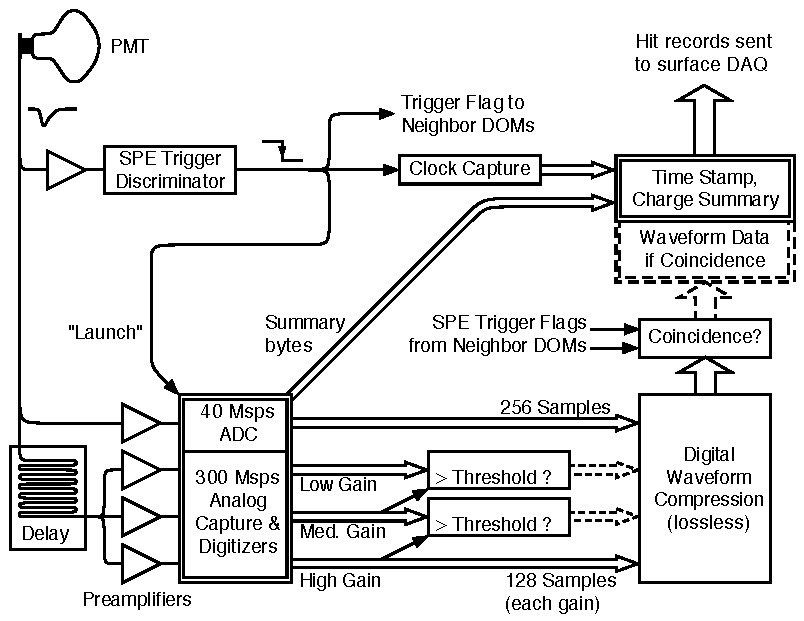
\includegraphics[width=0.9\textwidth]{graphics/dom/functional/domfig3-DOMDataFlow.pdf}
 \caption{Data flow diagram for recording and processing of PMT waveforms in the DOM to form 
 "Hit Records" that are sent to the surface DAQ computers.  As shown by dashes, full waveform data is only included
 when neighbor DOMs report time-coincident signals above the SPE discriminator threshold.  Additionally,
 data from low gain channels is omitted for waveforms that are within range of higher gain channels.}
 \label{fig:domdataflow}
\end{figure}

%NK section 3.5.2 text:
%Although low-power and high-speed, the ATWDs must be initiated by a trigger signal in order to start
%the digitizing operation. In order to capture the front pedestal of the waveform, the PMT signal is
%split in two ways: one branch enters the trigger circuit and initiates the ATWD and the other branch
%enters the delay line and emerges in the analog input of the digitizer after ?75 ns. The delay line
%is a stripline implemented as a ?10 m-long, 0.25 mm-wide, serpentine copper trace embedded in
%the dielectric and sandwiched between ground planes of the delay board. Unlike a coaxial cable
%delay line, the delay board is compact and easy to integrate into the limited space in the DOM
%sphere: the board is 3.2 mm thick and has the same area profile as the main board, below which
%it is mounted.
%(The impedance is 95 Ω. The delay time is 75±2 ns. The risetime and falltime is typically 3 ns
%(Including the source profile. ERD, Fig. 2). The signal attenuation is required to be less than 12\%.
%%The trace width was measured from ther gerber file. The trace length is based on the delay of
%0.166 ns per inch, found in the simulation file found on docushare, Document-6600.)

%%%%%%%%%%%%%%%%%%%%%%%%%%%%%%%%%%%%%%%%%%%%%%%%%%%%%%
%%[Below is more text that is too much detail for this paper]
%Several features are included for calibration functions of the DOM, also used for self-test.
%Each DOM has a local clock driven from a high-stability \unit[20]MHz(?) oscillator, in terms of which all local
%times are measured.  In order to determine slowly drifting offsets between clocks in each DOM and a master
%surface clock, the DOM provides waveform digitization of a regular timing pulse sent from the surface, as 
%well as sending a return pulse (Section~{sec:rapcal})~\cite{ref:domdaq}.
%For calibration of the waveform digitizers, the DOM has a pulser circuit that can inject programmed amounts of
%charge into the front end circuitry, and has an input multiplexer that allows the (adjustable) sampling rate
%to be calibrated via the clock oscillator.  
%A pulsed LED facilitates calibration of gain and time delay in the PMT as a function of applied high voltage 
%(Section~{sec:domcal}).

%During the first \unit[427]nsec recording interval, information is captured in one of two analog transient 
%waveform digitizers (ATWDs)
%with sampling period \unit[3.3]nsec, single bit resolution \unit[0.1?]mV for small signals and dynamic range
%\unit[7?]volts.  This period encompasses the time
%spread of most photons arriving from up to \unit[100]m away. 
%An analog delay line causes the recording to include a pretrigger period of at least \unit[10]nsec,
%allowing the leading edge to be measured with \unit[1]nsec resolution.
%For multi-photon pulses, the full arrival time profile can be reconstructed by fitting the waveform 
%as a sum of single photon responses, each contribution having typical amplitude
%\unit[5]mV and width \unit[12]nsec FWHM.
%The upper end of the dynamic range accommodates the full
%linear response range of the PMT, up to about 400(?) photoelectrons per \unit[15]nsec\cite{ref:pmtpaper}, 
%as well as fully saturated PMT pulses around \unit[5]volts amplitude.

%While the ATWDs are optimized for multi-photon events that are close to the DOM, the information
%content is more than needed for single isolated photon detections far away from the interaction,
%which may also be spread over a longer time period.
%Accordingly, the FADC is a separate 10-bit digitizer that records PMT waveforms for up to 
%\unit[6.4]{$\mu$sec} but with coarser sampling interval \unit[25]nsec.  
%This channel includes an anti-aliasing filter to broaden
%individual photon responses to \unit[70?]nsec FWHM and peak amplitude \unit[1]mV.
%With amplitude resolution \unit[0.1]mV, photon arrival times can still be determined to within \unit[7?]nsec.

%In order to quickly identify close-by events requiring full ATWD information, the cabling system includes
%extra wiring for DOMs to communicate directly with neighbors above and below~\cite{ref:domdaq}.  
%Each DOM trigger can 
%thus be quickly classified by whether a nearest or next-to-nearest neighbor DOM also
%triggered within a \unit[$\pm$1]$\mu$sec time window.  Such a local coincidence causes the full length
%ATWD and FADC waveforms to be saved, and otherwise only three FADC samples are saved along with
%the reference timestamp.
%%[End of text that is too much detail for this paper]
%%%%%%%%%%%%%%%%%%%%%%%%%%%%%%%%%%%%%%%%%%%%%%%%%%%%%%





\begin{figure}[h]
 \centering
 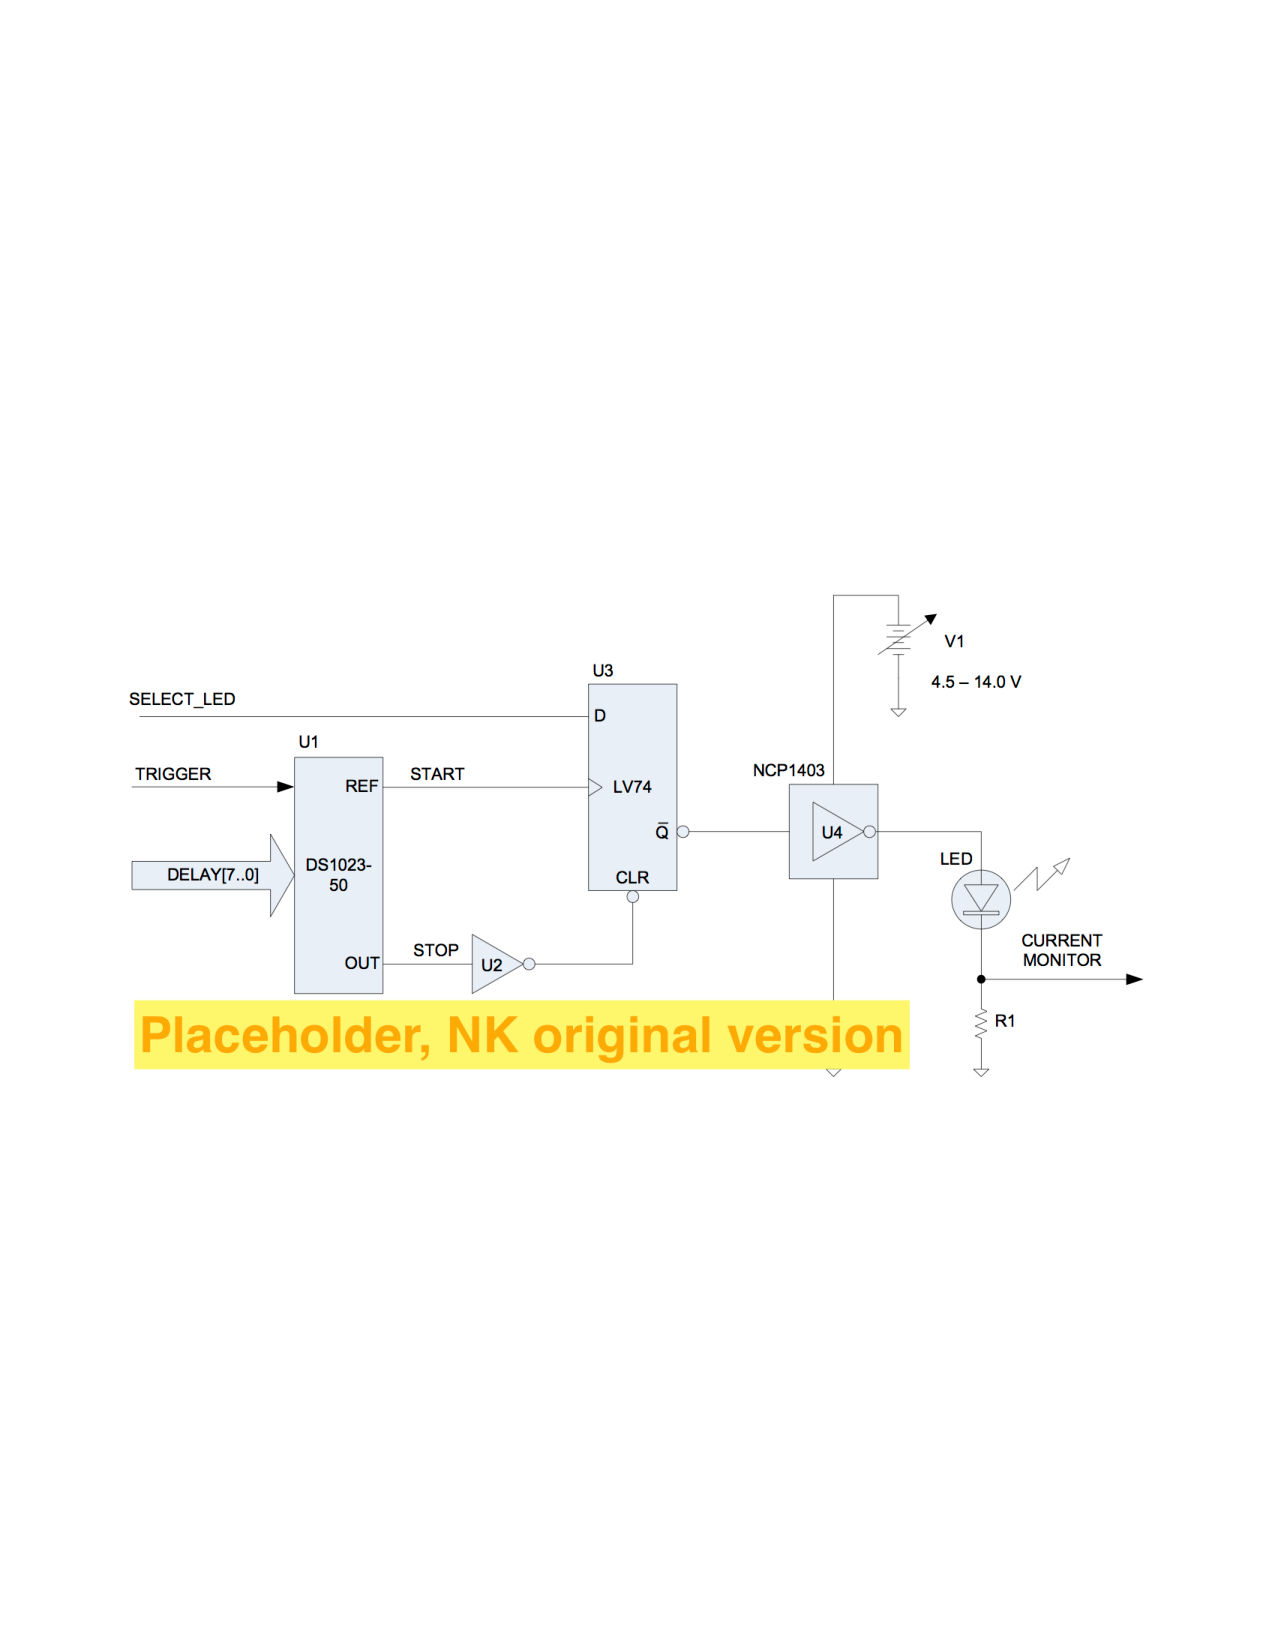
\includegraphics[width=0.6\textwidth]{graphics/dom/functional/domfig4-FlasherDiagram.pdf}
 \caption{LED flasher circuit diagram for one of twelve LEDs (simplified).}
 \label{fig:flasherdiagram}
\end{figure}

\begin{figure}[h]
 \centering
 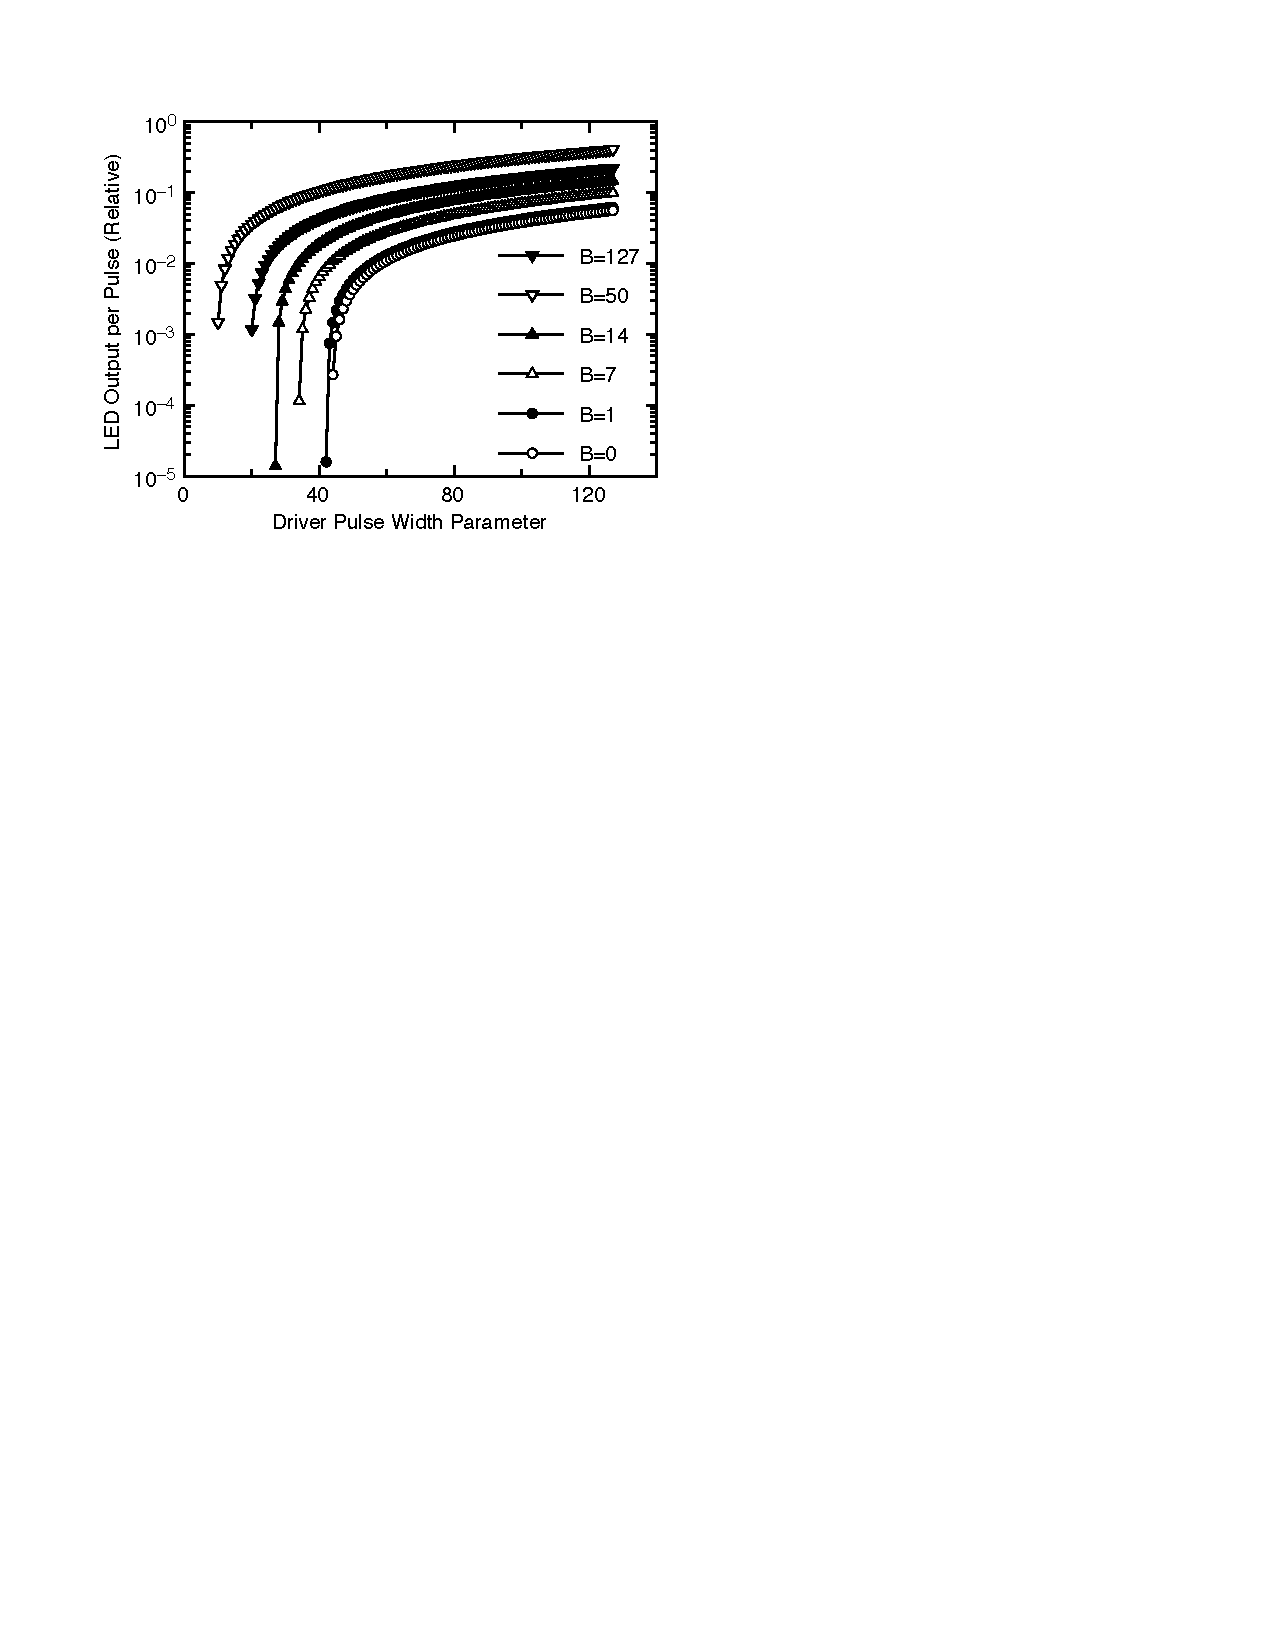
\includegraphics[width=0.6\textwidth]{graphics/dom/functional/domfig5-BrightnessModel.pdf}
 \caption{Light output from flasher LED pulses (relative to maximum), depending
on brightness and width configuration parameters.  Additional dynamic range is available
by enabling from 1 to 12 individual LEDs per DOM.}
 \label{fig:flasheroutput}
\end{figure}

\subsubsection{\label{sec:flasher}Flasher Board}

Each IceCube DOM contains a flasher board. The standard IceCube
flasher board, which is included in every DOM except the color DOMs
described below, is a circular board fitted with 12 LEDs (ETG-5UV405-30) 
specified with output wavelength \unit[$405\pm5$]nm.  Laboratory
measurements with sample DOMs showed a peak at
\unit[399]nm and spectral width \unit[14]nm (FHWM), which includes a
\unit[$-1$]nm shift when operating at low temperature.
The LEDs are arranged in pairs, evenly spaced around the board
with a 60$^{\circ}$ separation between each pair. One LED in each pair
points outward horizontally and the other is tilted upward at an angle
of 48$^{\circ}$, close to the Cherenkov angle in ice ($n=1.317$). 
The angular emission profile of each LED has a FWHM of
30$^{\circ}$ in air, which is modeled as a Gaussian emission profile
with $\sigma = 13^{\circ}$. After refraction through the DOM glass and into
the ice, the value of $\sigma$ is 9.7$^{\circ}$ in the polar direction
and 9.8$^{\circ}$ in the azimuthal direction for the tilted LEDs, and  9.2$^{\circ}$ in the polar direction
and 10.1$^{\circ}$ in the azimuthal direction for the horizontal LEDs.
About 10\% of the light is emitted outside the Gaussian beam, modeled by
a profile proportional to $(1+\cos{\alpha})$ where $\alpha$ is the angle away from the LED axis.


The LEDs are controlled by a current pulse applied to each LED through
a high speed MOSFET driver with a series resistor (Figure~\ref{fig:flasherdiagram}). 
The LEDs can be enabled individually or in any
combination of the 12, by setting bits in a configuration parameter.
The photon output of each LED depends on the width and
amplitude of the driving current pulse, which are controlled as common
values for all enabled LEDs in each DOM (Figure~\ref{fig:flasheroutput}).  
The pulse width parameter (0-127) controls width up to a maximum of \unit[70]{nsec}; 
for sufficiently short driving current pulses the light output narrows to \unit[6]{nsec} (FWHM) with
10\% afterglow decaying over \unit[15--20]{nsec}.
The brightness parameter (0-127) controls the driving voltage between $4.5$ and \unit[15]{volts}, yielding
peak current up to \unit[300]{mA}.
By varying brightness and width settings as well as the number of LEDs enabled, DOMs can generate flashes
from $10^6$ to $1.4\times10^{11}$ photons, similar to the total light from
neutrino interaction cascades between \unit[7]GeV and \unit[1]PeV energy.
The low end of this dynamic range requires fine tuning of driving parameters because of
operating LEDs very close to threshold.

The LED current waveforms are recorded in an auxiliary ATWD channel, supplying
a rising edge time that also establishes the onset of the optical pulse (after a known
turn-on delay).
The repetition rate is programmable up to \unit[610]{Hz}.
Although flashers can be
operated in multiple DOMs in the same run, the DAQ does not support
time-synced flashing of LEDs on different DOMs, so coincident flasher
events happen only by chance. 

The flasher LEDs are used for a variety of calibration purposes:
\begin{itemize}
\item verifying the timing response of the DOMs throughout the
  software
\item measuring the position of the deployed DOMs in ice
\item measuring the optical properties of the ice
\item verifying the performance of cascade reconstruction algorithms
  in measuring position, direction and energy
\end{itemize}

{\it Color DOMs}

There are 16~DOMs (8 on string~79 in the center of IceCube, 8 on
string~14 on the edge of IceCube) fitted with multiwavelength flasher boards, called
color DOMs or cDOMs. Each cDOM includes 3 LEDs with a nominal
wavelength of 505~nm, 3 LEDs with a nominal wavelength of 450~nm, 3
LEDs with a nominal wavelength of 370~nm and 3 LEDs with a nominal
wavelength of 340~nm. The LEDs are arranged in pairs as on the
standard flasher board, but all LEDs point outward horizontally. 
The properties of the LEDs are given in
Table~\ref{table:cdom_properties}.

\begin{table}
\caption{Properties of the cDOM LEDs}
\begin{tabular}{|c|c|c|c|c|c|c|}
  \hline
 LED& nominal $\lambda$ & measured $\lambda$ & $\sigma$ air & $\sigma$
 DOM, polar & $\sigma$ DOM, azimuthal \\
\hline
UVTOP335-FW-TO39 &340 nm&338 nm&	51.0$^{\circ}$ &	36.1$^{\circ}$ &	42.9$^{\circ}$\\
\hline
NS370L\_5RFS &370 nm&	371 nm&55.2$^{\circ}$&	39.1$^{\circ}$&	42.9$^{\circ}$\\
\hline
LED450-01 & 450 nm& 447 nm&	6.8$^{\circ}$ &	4.8$^{\circ}$ &	5.3$^{\circ}$ \\
\hline
B5-433-B505 & 505 nm& 494 nm& 6.4$^{\circ}$ &	4.5$^{\circ}$ 	&4.9$^{\circ}$ \\
\hline
\end{tabular}
\label{table:cdom_properties}
\end{table}

\subsection{\label{sec:dom_prodtest}  Production and Testing}

DOM Integration and Test had some clear objectives as the IceCube project
moved from the instrumentation design stage to the production and
installation at the Pole phase of the project’s construction. One,
approximately 5500 in-ice and IceTop DOMs were required to be built, tested
and delivered to the South Pole. Two, all of the DOMs must meet the
stringent quality requirements needed for them to work reliably buried deep
in the ice for more than 20 years of lifetime. Finally, this work must be
done such that the DOMs were delivered on time, within budget and that they
meet all technical specifications. The IceCube project’s principal
bottleneck for delivering science was the hot water drilling to be done
each austral summer at the South Pole. It was critically important that
drilling never stopped on account of an instrumentation inventory shortage
of any kind. The instrumentation needed to deploy into each successfully
drilled hole to be ready. This dictated a DOM Production strategy that was
based on electronics manufacturing best practices and a team that was
committed to success. Additional challenges included lack of electronics
manufacturing infrastructure within the IceCube Collaboration, multi-site
production, cultural differences, South Pole logistics chain and an
unpredictable project funding profile. The DOM Production plan was
implemented in a 3-stage approach. Stage 1 was to produce 400 DOMs at the 3
DOM production sites. This was a sufficient quantity to supply
instrumentation for the 1st year drilling plan of 4 holes at Pole and to
verify DOM production readiness at all locations. It also allowed for the
DOM design to be verified as good after a deployment season. If major
design problems were discovered, they could be addressed before significant
material supplies were purchased. Stage 2 was the procurement of materials
and supplies for another 1000 DOMs. Lastly, the last stage procurements
were done for the remaining 4100 DOMs to be integrated and tested.

The planning stage for DOM Production was when the manufacturing
infrastructure was installed at the 3 DOM Production sites. It was
organized in 5 areas of focus: Methodology, Materials, Labor, Equipment,
and Environment. Methodology referred to the actual process flow to
integrate and test a DOM. The process flow was required to be fixed so it
could be successfully transferred to each site. A DOM Process Traveler was
created which listed each process step required. In addition, the date,
technician and material serial numbers were recorded onto the Process
Traveler. All the information was then entered into a central DOM
Production database. Each DOM was to be individually tested and its data
reviewed by someone independent of the production team prior to shipment to
Pole. Materials required for DOM integration and test was listed in the
controlled document called Bill of Materials. Sole source procurements were
identified early and executed. Suppliers were actively managed during DOM
Production with regular visits to the vendor sites. It was expected that
all materials were fully tested at the supplier sites and were delivered to
the DOM production sites Certificates of Conformance indicating that the
materials were acceptable for use in the DOM production environment. Some
materials, such as the PMT and sphere, were directly drop shipped to the
DOM production sites. Everything else was shipped to the US DOM production
site (Physical Sciences Laboratory (PSL), Stoughton, Wisconsin) where they
were kitted for delivery to the 2 European DOM Production sites (DESY,
Zeuthen, Germany and Stockholm University, Sweden). Discrepant materials
discovered during the manufacturing process were segregated and
dispositioned accordingly via a rigorous Quality Control system. Total
material purchases were made so that the ending material inventory was very
small. The intent was for all materials to be converted into working
DOMs. Labor was planned at each site for continuous DOM production. All
technicians were trained and certified to perform integration and test
tasks. Each site had separate Quality function personnel. Equipment used
for DOM integration and test was the same at all sites. It was either made
custom per specified drawings at each site or was made at PSL and shipped
to DESY and Stockholm University for use. All jigs were qualified for use
prior to introduction in the manufacturing process. Measurement equipment
was calibrated and records maintained that verified their traceability to a
reference standard. DOM integration took place in an ESD, temperature and
humidity controlled environment. Separate areas were established for
inventory storage, Work in Process (WIP), non-conforming materials and
finished DOMs ready to ship. Each integration site was kept very clean to
minimize the introduction of contaminants that might result in failed
components. Finally, each of the 3 DOM production sites had to be qualified
for production by passing a rigorous inspection. In summary, the
introduction of manufacturing protocols based on electronics industry best
practices allowed for each site to be independent yet produce DOMs that
were form, fit and function identical. Weekly phone calls each week between
the sites tracked progress and performance. 

The actual DOM integration and test process was composed of 18 discrete
steps tracked via the Process Traveler. The first 15 steps related to
integration while the last steps were concerned with Final Acceptance
Testing (FAT), DOM harness attachment and final packing procedures needed
before shipping to the South Pole. The integration process started with the
PMT Collar attachment to the PMT. The PMT Collar provided a mounting point
for the electronic boards needed inside a DOM. The PMT was then mounted
into a special jig that allowed for precise placement inside the bottom
glass hemisphere. In parallel, the mu metal shield  was placed inside the
bottom hemisphere and a silicone dielectric gel was mixed and poured into
the same hemisphere. The gel was then degassed. After degassing, the PMT
was placed in the gel and it was allowed to cure for 48 hours before
further processing. After curing, the PMT High Voltage Base was soldered
onto the flying leads of the PMT. Separately, the PC Board stack was made
by attaching the Delay Board, Main Board, Flasher Board and High Voltage
Control Board together with screws and standoffs. After PC Board stack
assembly, it was mounted onto the PMT collar and attached with 3 small
screws. The penetrator assembly was mounted into the top hemisphere and the
two halves of the sphere were brought together so the penetd functionality
was confirmed to be good before the DOM moved to Final Acceptance Testing
(FAT).

All DOMs at all sites were required to pass a rigorous testing protocol at
cold temperatures in a dark environment before shipping to the South
Pole. The testing was done in Dark Freezer Labs (DFLs) that were maintained
at each production site. In addition to acceptance testing, individual DOM
characterization was done to inform future physics analyses. The main
functional test was called the Simple Test Framework (STF) which was a
self-diagnostic functional test installed on each Main Board. DOM
Calibration (DOMCal) was also performed along with local coincidence
testing. The tests were done at various temperatures during the typical 22
days in the DFL (see Fig.~\ref{fig:fat_cycle}). A key element in FAT was to compare testing
results at the beginning of the testing with those attained at the final
room temperature test. Major changes in parameters were flagged as
potential problems and were dispositioned accordingly. Approximately xx
performance parameters were evaluated and measured during FAT. The typical
first pass rate for DOMs during FAT was approximately 90\% (check
this). After the successful completion of FAT, DOM deployment harnesses
were attached and the DOMs individually packed in custom cartons that were
then combined into overcartons that held 8 DOMs ready for shipment. DOMs
were additionally tested on the ice at the South Pole prior to deployment
into the ice. This was done to ensure DOMs did not sustain any damage as a
result of a strenuous journey to Pole. Eight overcartons were placed on a
custom sled that allowed for testing of 64 DOMs at a time. They were
covered with an additional cover that helped block any light from reaching
the DOMs in their packaging. STF testing was done along with a measurement
of dark rates before final installation into the holes. Of the
approximately 5500 DOMs shipped to Pole, about 30 were shipped back to the
US after failing on-ice testing.    

\begin{figure}[!h]
 \centering
 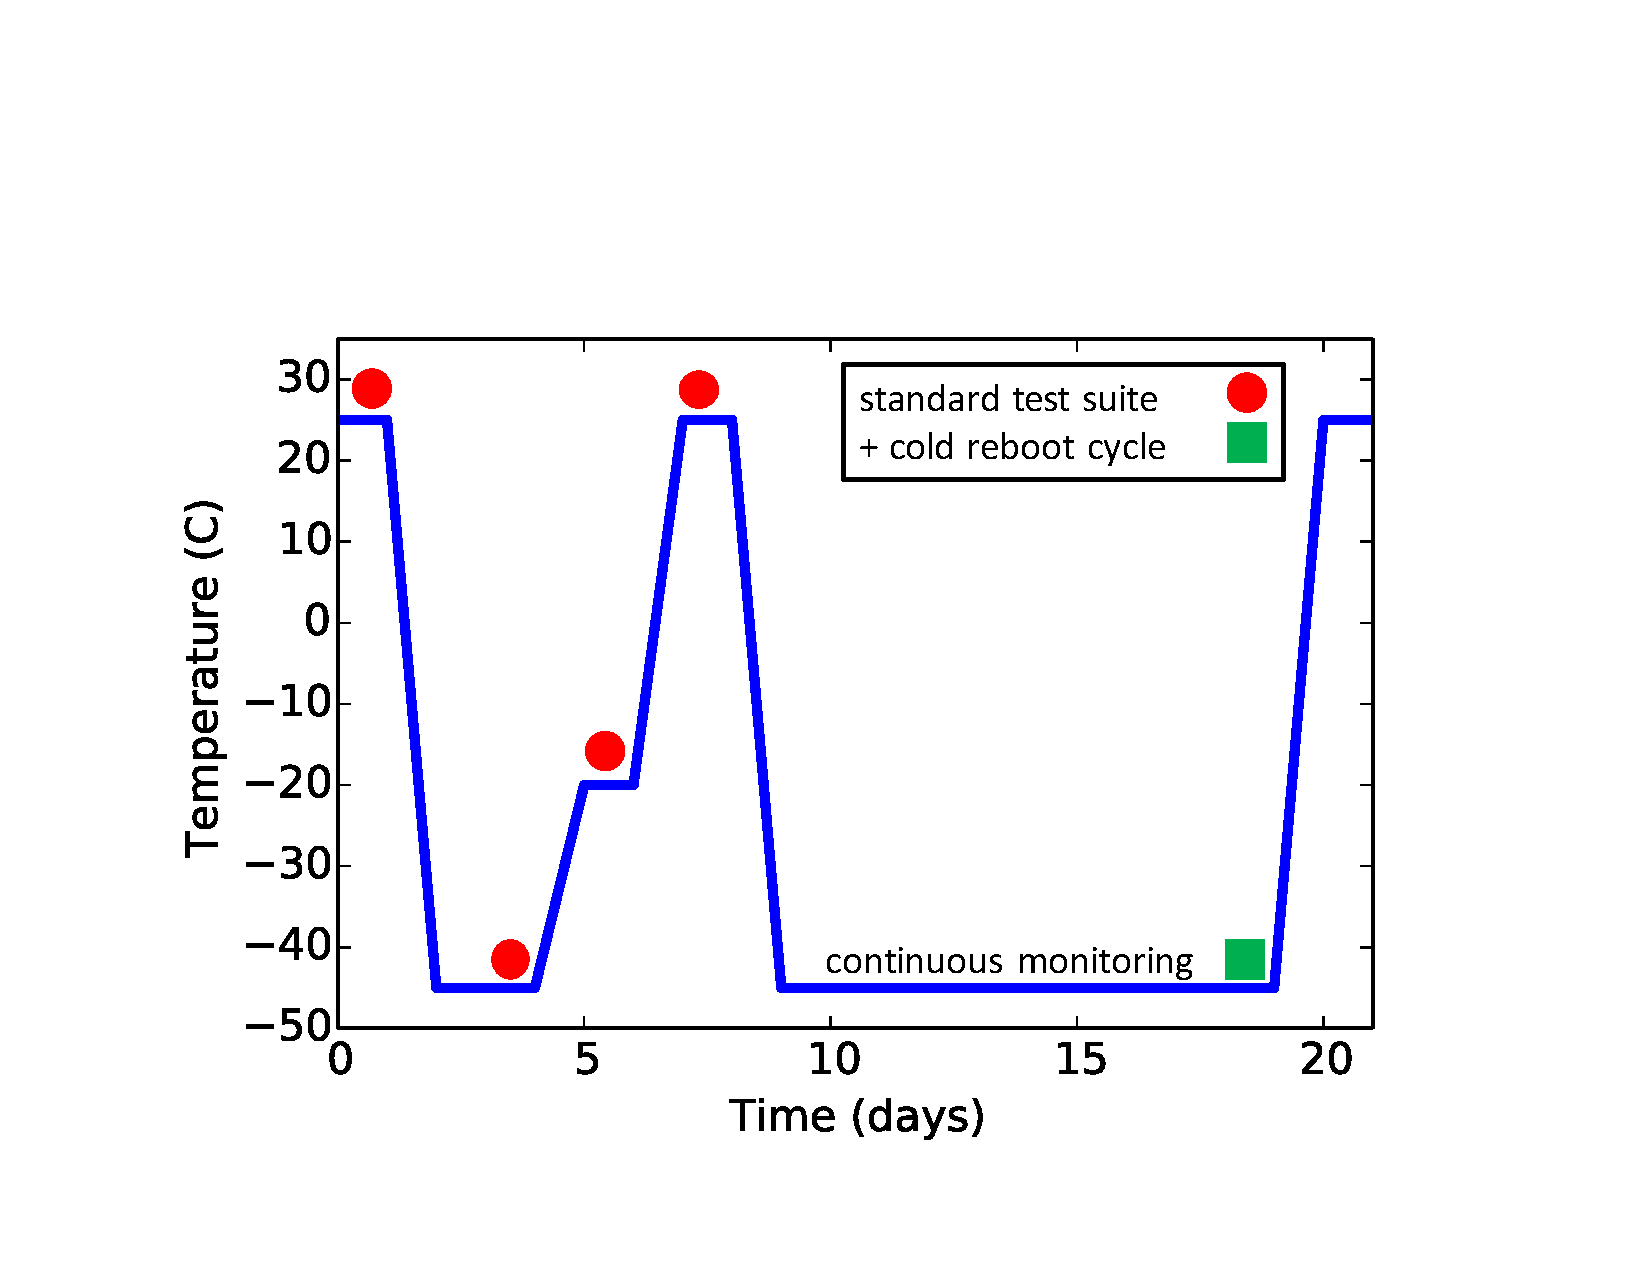
\includegraphics[width=0.9\textwidth]{graphics/dom/production/fat_cycle.pdf}
 \caption{Final Acceptance Test (FAT) temperature profile, including
   testing steps performed at each stage.}
 \label{fig:fat_cycle}
\end{figure}

\subsection{\label{sec:dom_calibration}  Calibration}

\subsubsection{\label{sec:domcal} DOMCal}

The calibration of the PMT waveforms recorded by the DOMs, i.e. translation
of digitized samples into voltage and time, as well as the gain of the PMT
itself, is achieved via DOM-by-DOM calibration constants determined by the
modules themselves.  The calibration software, DOMCal, uses precision calibration
circuits on the DOM Main Board as well as single photons as inputs
for a ladder of calibration routines.  Analysis and fitting of the
calibration results is done by the DOMCal software, with the results being
transmitted from each DOM to the surface as an XML file of fit parameters.

%The ladder of calibration routines is shown in
%Fig.~\ref{fig:domcal_ladder}.
The primary reference inputs to the calibration are a precision electronic
pulser circuit providing known charges; a circuit providing a reference DC
bias voltage level; the 20 MHz oscillator on the Main
Board, used as the timing reference; and single photoelectrons, either from
ambient ``dark noise'' photons or a low-luminosity LED on the Main Board.

Because the operating conditions for
the in-ice DOMs are so stable, DOMCal is only run once a year on the full
detector. IceTop DOMs are calibrated once per month.  Calibration is
typically performed on half the detector at at time, the other half
remaining in data-taking mode.  Because the calibration procedure produces
light, however, these runs are not used in normal analysis.

% FIX ME: ATWD reference?

First, the discriminator circuits used to trigger the DOM are calibrated
using the electronic pulser circuit.  This calibration is later refined using actual
PMT waveforms, once the PMT gain is known.  Next, the ATWD voltage levels
are calibrated by sweeping the input DC bias voltage and recording the
response; because of the slight variations in the ATWD circuits, this
calibration is produced for every sample and every channel.

This ATWD calibration also in principle allows determination of the baseline
voltage levels of each channel, needed for charge integration.  However, in
practice, these baselines are extremely sensitive to the operation
condition of the DOMs, and since data-taking conditions cannot be exactly
replicated while running DOMCal, the baselines used during data-taking are
determined instead by using averaged forced triggers taken during a normal
run.  DOMCal can still use its own baselines, though, for charge integration
during the calibration procedure.

The highest-gain channels of the two ATWDs are calibrated using the electronic
pulser circuit, and then the gains of the other ATWD channels and the FADC
are determined by varying the pulser output and comparing the charges
simultaneously recorded in multiple gain channels.  This relative
calibration is later refined using PMT waveforms stimulated by the Main
Board LED.

The ATWD sampling speed is calibrated by digitizing the Main Board oscillator
waveform and recording the number of clock cycles as a function of ATWD
speed setting.  The FADC sampling speed is slaved to the 20 MHz
oscillator, which is used as a timing reference.  The relative timing of
the ATWD and FADC waveforms is determined using the electronic pulser circuit;
non-linear fitting of the digitized waveforms to known templates is
required in order to determine the FADC offset to the required accuracy.
The transit time of the PMT and delay board as a function of PMT high
voltage is determined by calculating the delay between the digitized
current pulse through the Main Board LED and the observed light pulse in
the ATWDs.   

The PMT gain as a function of high voltage is calibrated using ambient
``dark noise'' photons --- the charge $e$ prior to amplification is quantized
and known.  At each voltage level, a histogram of many waveform charges is recorded,
and each histogram is fit with an exponential plus Gaussian model (see
Fig.~\ref{fig:domcal_hvfit}).  The peak of the Gaussian component is used to
determine the amplification of the PMT at each voltage, and a linear fit
of $\log_{10}(\mathrm{gain})$ versus $\log_{10}(\mathrm{voltage})$ allows
the high voltage of each PMT to be tuned to desired operating point ($10^7$
for in-ice DOMs; see Fig.~\ref{fig:domcal_hv_settings}).  Small ($3-5\%$)
corrections to the gain of each DOM are determined using charge
distributions recorded during normal data-taking; this corrects for a small
systematic difference in the charge as determined by DOMCal's integration
and the waveform pulse unfolding used in data processing.

% From JK DOMCal Hist.ipynb
\begin{figure}[!h]
 \centering
 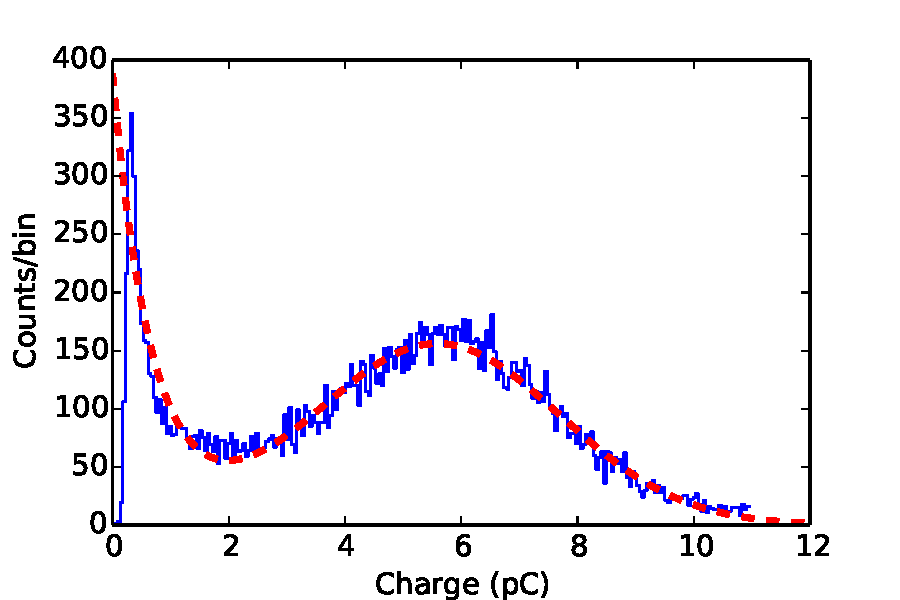
\includegraphics[width=0.6\textwidth]{graphics/dom/domcal/hvfit.pdf}
 \caption{Sample SPE charge spectrum as recorded by DOMCal and fit
   \textit{in situ} with a Gaussian+exponential model.} 
 \label{fig:domcal_hvfit}
\end{figure}

% From JK DOMCal HV Settings.ipynb
\begin{figure}[!h]
 \centering
 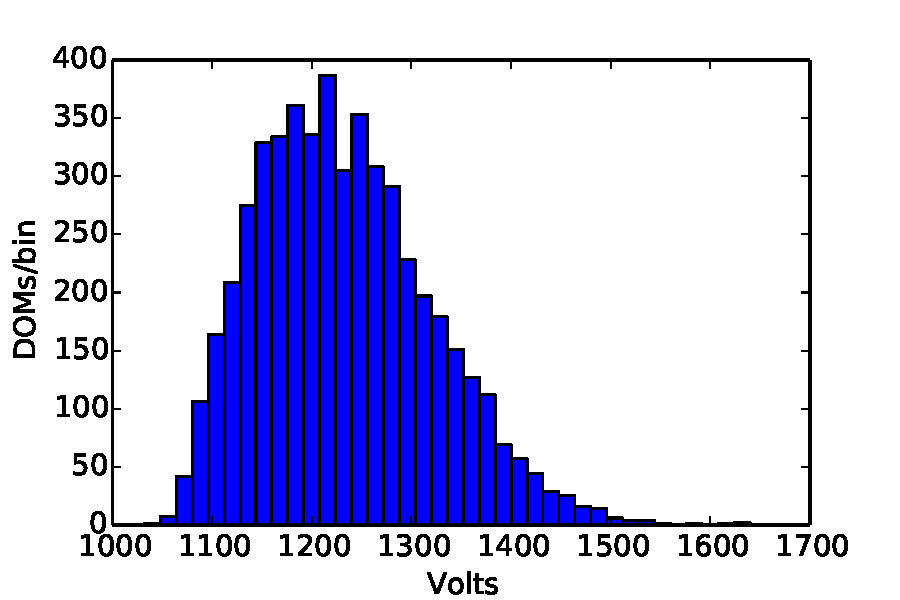
\includegraphics[width=0.6\textwidth]{graphics/dom/domcal/inice_hv_2016.pdf}
 \caption{PMT high voltage at $10^7$ gain for in-ice DOMs.}
 \label{fig:domcal_hv_settings}
\end{figure}

\subsubsection{\label{sec:waveformcal} Waveform Calibration and Droop
  Correction}
An ATWD waveform consists of readouts from 128 independent digitizers,
while an FADC waveform consists of successive outputs of a 6-stage
pipelined digitizer (3 bins for SLC launches and 256 for HLC
launches). Two calibration constants are needed to turn each of these
raw digitizer readout values (an integer number of ADC counts) into a
voltage, from which the deposited charge is calculated. The deposited
charge is the basis for all energy measurements in IceCube. The
calibration constants needed are 1) the pedestal, the value the digitizer reads when the input voltage is zero, and
2) the gain, the input voltage required to increase increase the readout value by one count. 

Since each bin of each ATWD channel is read from an independent
digitizer, it is important to distinguish between the pedestals of
individual bins and the common pedestal of the entire waveform. The
baseline is the mean of the pedestals of each bin in a waveform. For
the FADC, this is the same as the pedestal. The pedestal pattern is
the deviation of each bin's pedestal from the common baseline. For the
FADC, this is identically zero. Since 2008, the DOM has subtracted the
pedestal pattern from
the ATWD waveform before sending it to the surface. The pedestal pattern is computed at the beginning of each
run by comparing 25 averaged pedestals. The autocorrelation coefficent
between the pairs of averaged pedestals is computed to detect light
contamination in the pedestals, and the shift between the baseline of
the pairs is calculated to determine that the baseline is stable. This
procedure ensures that fewer than 1 DOM in 1000 runs will contain a
contaminated baseline. Thereafter, both ATWD
and FADC waveforms can be calibrated by first subtracting the common
baseline from each bin, then multiplying by the gain. Correct
measurement of the common baseline is critical to correct charge
measurement and energy reconstruction.

The baseline is set to about 10\% of the maximum value of the
digitizer counts in
order to capture signals that go below the baseline. Since 2012, the baseline value is set by the DAQ configuration in order to ensure
stability. The baseline value differs for each digitizer channel in
each DOM, ranging from 112 to 161 counts in the fACD and 109 to 172
counts in the ATWD. The baselines for each digitizer channel in each DOM are measured with
beacon hits, forced triggers which are collected at a rate of 1.2~Hz
per DOM
in in-ice DOMs and 4.8~Hz in IceTop DOMs. Beacon waveforms
from the FADC and ATWD of a typical DOM are shown in Figure~\ref{fig:raw_baselines}.

\begin{figure}[!h]
  \captionsetup[subfigure]{labelformat=empty}
  \centering
  \subfloat[]{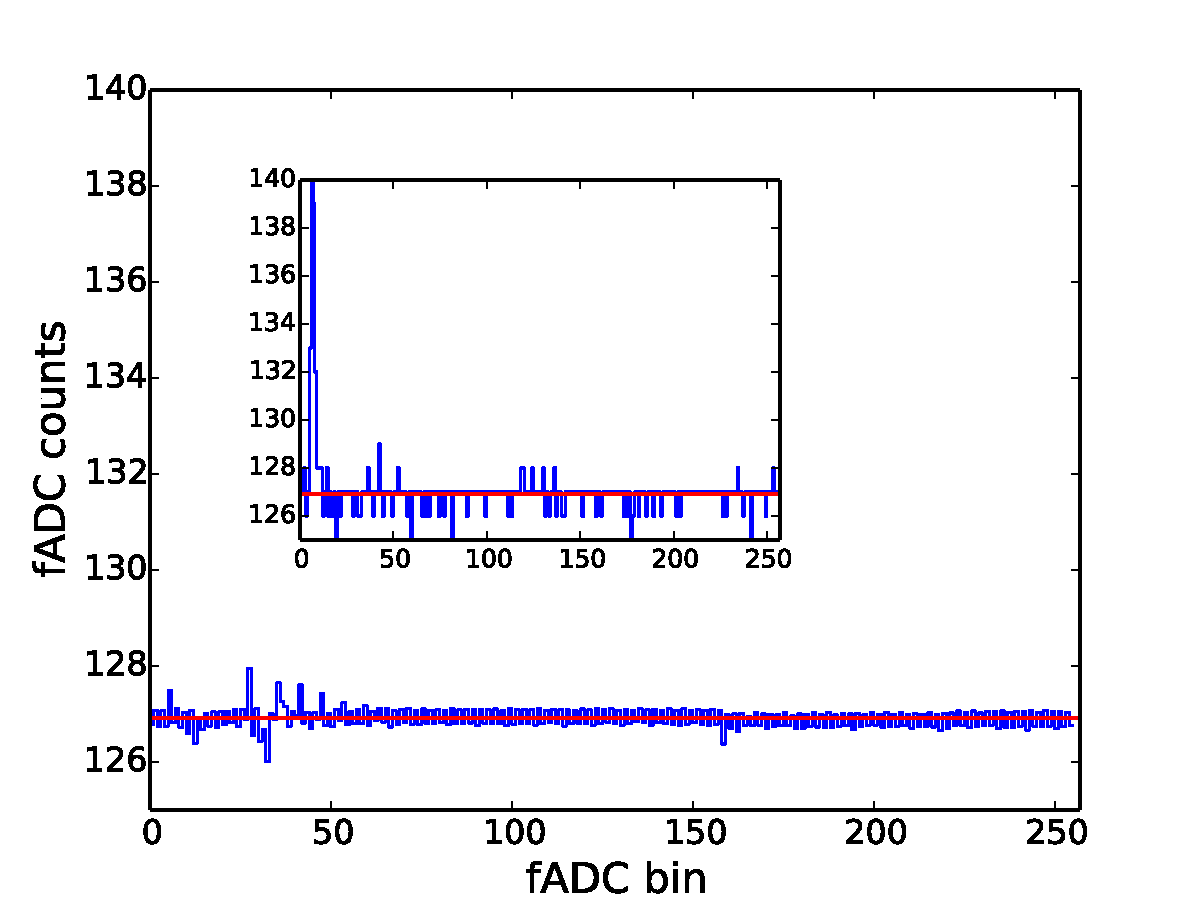
\includegraphics[width=0.5\textwidth]{graphics/dom/reliability/fadc_average_beacon_raw.pdf}}
  \subfloat[]{\includegraphics[width=0.5\textwidth]{graphics/dom/reliability/ATWD_average_beacon_raw.pdf}}
  \caption{Beacon waveforms from the FADC (left) and ATWD (right) of
    an IceCube DOM. The waveforms are an average of about 1000 beacon
   launches. The baseline, which is the mean value of the
    beacon waveform, is shown as a horizontal red line. Typical raw SPE
    waveforms are inset.}
  \label{fig:raw_baselines}
\end{figure}

The gain is measured by DOMCal (Sec.~\ref{sec:domcal}), a single value
for the FADC waveform and a bin-dependent value for the ATWD
waveform. The calibrated waveform voltage is then

\begin{equation}
  \mathrm{voltage} = \mathrm{(ADC  counts - baseline)*gain}
\end{equation}

The waveform start time is then corrected for the PMT transit time,
the average time it takes a pulse to propagate through the entire
PMT. The PMT transit time correction $t_{transit}$ is dependent on the PMT high
voltage:

\begin{equation}
  t_{transit} = \frac{m}{\sqrt{HV}} + b
\end{equation}

where $m$ and $b$ are determined by DOMCal. The typical value of $m$
is 2000~ns$\cdot \sqrt{\mathrm{V}}$ and the typical value of $b$ is
80~ns, which includes the 75~ns delay line of the mainboard. The
typical transit time is therefore 130~ns. 

Waveform start times from the second ATWD chip and the FADC are further
corrected for the delay $\Delta t$ with respect to the first ATWD
chip, so the total start time correction is $t_{transit} + \Delta t$.

Finally, the waveforms are corrected for the effects of droop from the
transformer that couples the mainboard to the PMT output. The toroid
coupling effectively acts as a high-pass filter on the PMT output
which makes the tails of the waveforms ``droop'' and even
undershoot. This effect is temperature dependent and is worse at lower
temperatures. The droop correction inverts the effect of the high-pass
filter and eliminates the undershoot in the waveform tails. This is
done by calculating the expected reaction voltage from the toroid at
each time, and adding the reaction voltage to the calibrated waveform
to compensate. The reaction voltages are made to decay exponentially
according to a temperature-dependent model of the transformer’s
behavior. When a readout contains consecutive launches from the same
DOM, the reaction voltages at the end of the last launch are used to
correct for the residual droop in the follow-on launch. IceCube DOMs
use two types of toroid transformers: the ``old toroid'' with a short
time constant which was used in early DOM production, and a ``new
toroid'' with a longer time constant that produces less
distortion. The  full correction is modeled with a dual time constant
where the DOM's transient response $\tilde{\delta}(t)$ to an input
signal $\delta(t)$ is given by

\begin{equation}
\tilde{\delta}(t) = \delta (t) - N((1 - f) e^{t/\tau_1} +f
e^{t/\tau_2})
\end{equation}

The first time constant $\tau_1$ is given by 
\begin{equation}
\tau_1(T) = A + \frac{B}{1 + \exp{-T/C}}
\end{equation}
where $T$ is temperature and $A$, $B$ and $C$, $N$ and $f$ are determined empirically.

For old toroid DOMs, the second time constant $\tau_2 =
0.75\tau_1$. For new toroid DOMs, the second time constant is 500~ns. 

\subsubsection{\label{sect:dom:rapcal}RAPCal}

The Reciprocal Active Pulsing calibration (RAPCal) is a
continuously-running method for translating hit timestamps from the the
individual free-running DOM clock domains to the clock domain in the
IceCube Lab, which is synchronized to UTC.  A bipolar pulse is sent to each
DOM over the power/communications wire pair and then returned, with each
transmission and receive point timestamped locally.  The symmetry of the down-
and up-transmission allows a translation from each DOM clock domain to the
surface clock domain at the midpoint, without prior knowledge of cable lengths.
The base implementation is described in Ref.~\cite{ICECUBE:DAQ}; we
describe here the details of the time translation algorithm and validation
of the DOM relative synchronization. 

\begin{figure}[!h]
 \centering
 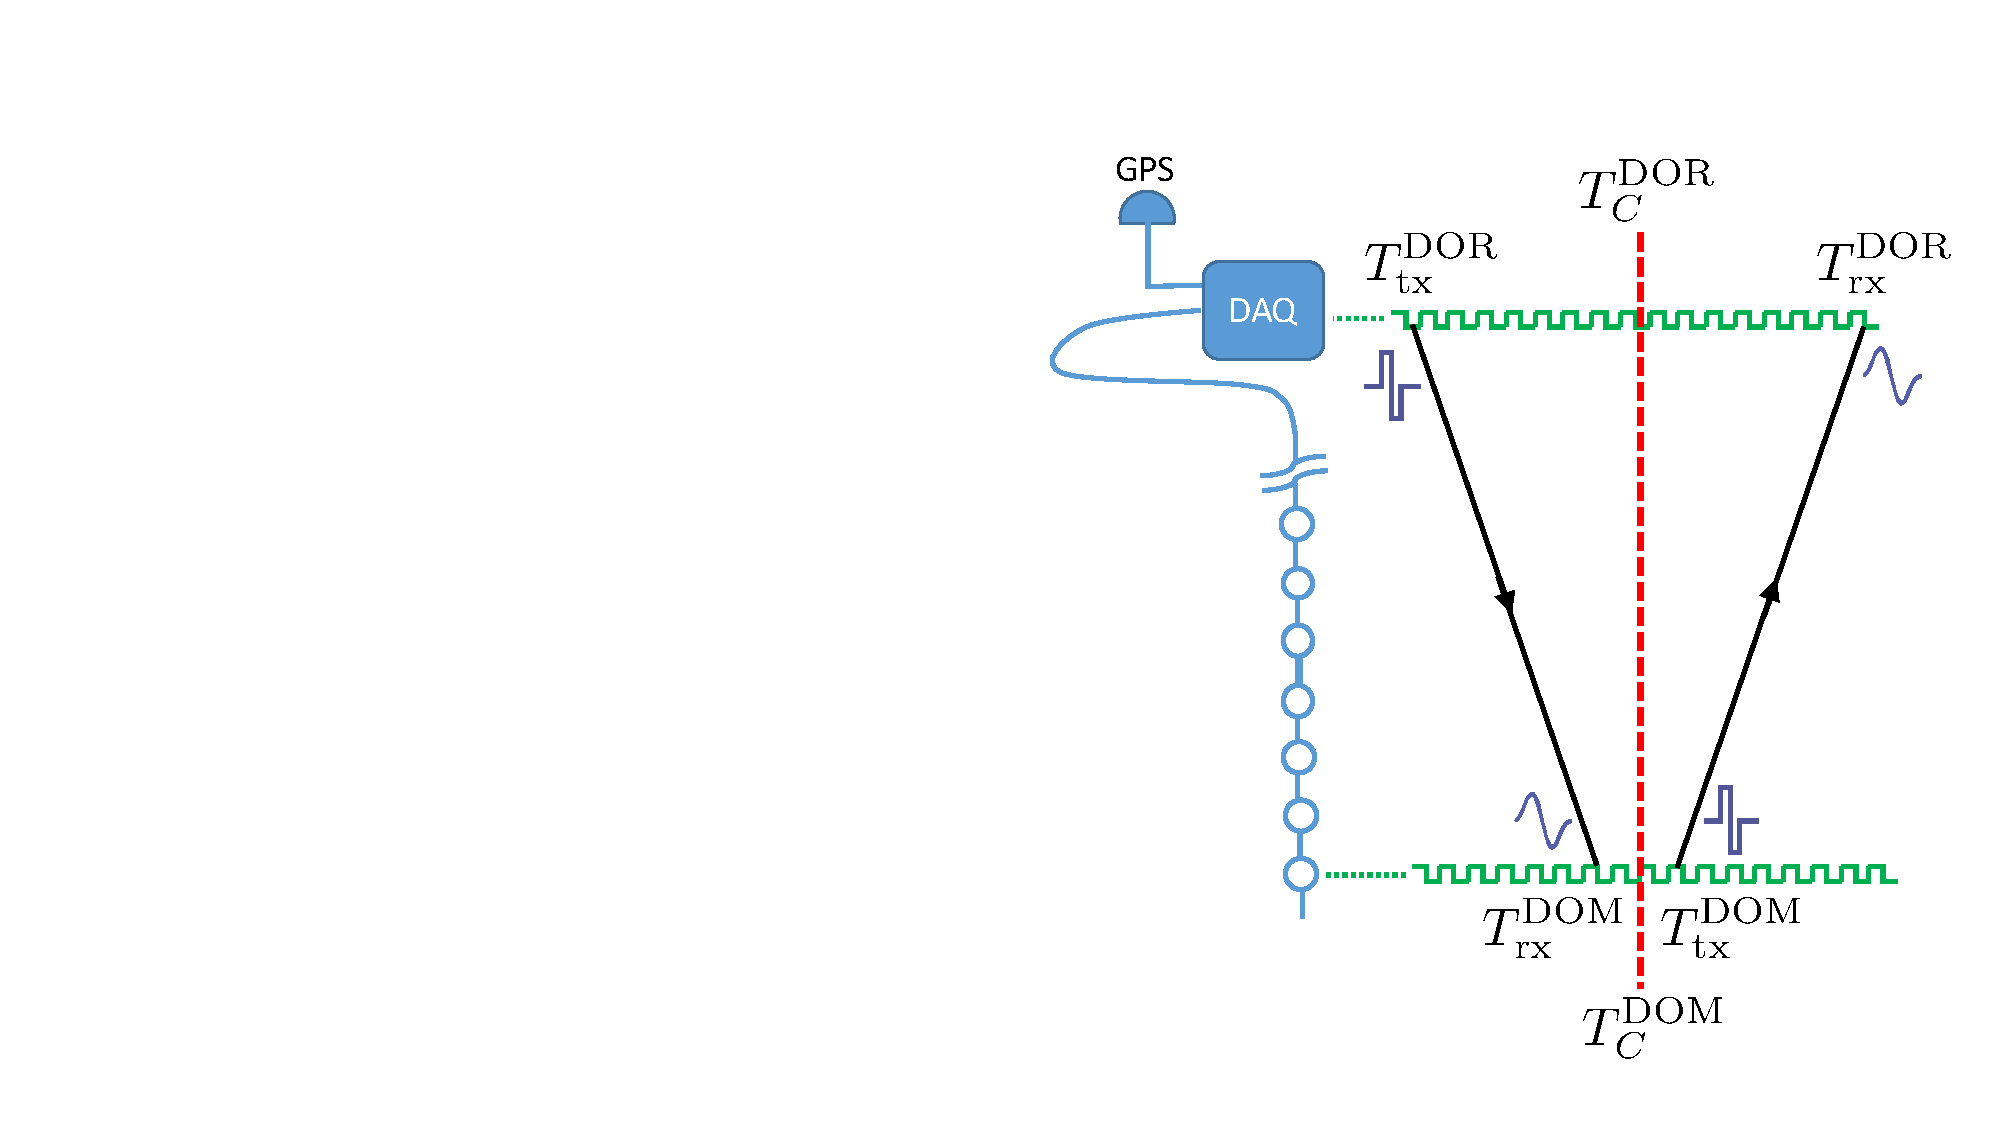
\includegraphics[width=0.4\textwidth]{graphics/dom/rapcal/rapcal_symmetry.pdf}
 \caption{The Reciprocal Active Pulsing calibration (RAPCal) allows
   translation from the free-running clocks of each DOM to the GPS-slaved
   clocks in the IceCube lab.  Each transmit and receive pair is
   timestamped in the local clock domain, and by the symmetry of the
   situation the midpoints are synchronous.}
 \label{fig:rapcal_symmetry}
\end{figure}

\begin{figure}[h]
 \centering
 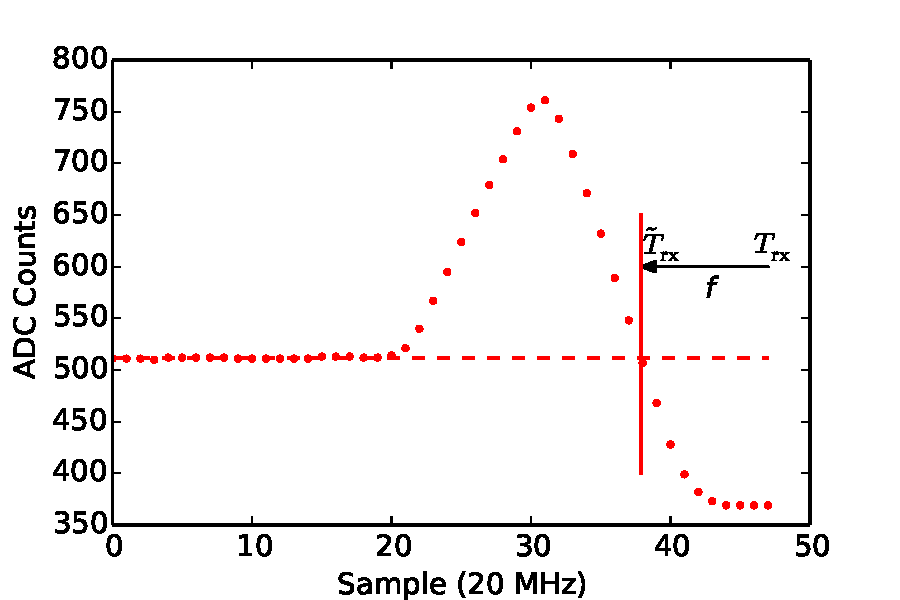
\includegraphics[width=0.6\textwidth]{graphics/dom/rapcal/dom_wf_zero_crossing.pdf}
 \caption{Digitized RAPCal pulse as received by a DOM, after cable dispersion.  The
   zero-crossing of the baseline-subtracted pulse is used as a fine-delay
   correction to the received timestamp.}
 \label{fig:rapcal_zero_crossing}
\end{figure}

A RAPCal pulse sequence to each DOM results in a series of four timestamps
$T_{\mathrm{tx}}^{\mathrm{DOR}}$, $T_{\mathrm{rx}}^{\mathrm{DOM}}$, 
$T_{\mathrm{tx}}^{\mathrm{DOM}}$,  and $T_{\mathrm{rx}}^{\mathrm{DOR}}$
(Fig.~\ref{fig:rapcal_symmetry}), with timestamps in 20 MHz units
of the DOM and surface (DOR, see Sect.~\ref{sect:online:master_clock}) clocks.  The received dispersed bipolar pulses
are digitized by the communications ADCs and 
timestamped.  A ``fine delay'' correction $f$ to
$T_{\mathrm{rx}}^{\mathrm{DOM}}$ and $T_{\mathrm{rx}}^{\mathrm{DOR}}$ is calculated by interpolating
to find the negative-going zero crossing, relative to a baseline voltage
calculated using the initial samples of the waveform (Fig.~\ref{fig:rapcal_zero_crossing}):

\begin{equation}
  \tilde{T}_{\mathrm{rx}} = T_{\mathrm{rx}} - f\ .
\end{equation}


\noindent The midpoints $T_C^{\mathrm{DOR,DOM}}$ halfway between $T_\mathrm{tx}^{\mathrm{DOR,DOM}}$ and
$\tilde{T}_\mathrm{rx}^{\mathrm{DOR,DOM}}$ are identified as synchronous.

To translate an arbitrary DOM timestamp $t$ to UTC
time, we use the RAPCal results bracketing $t$ to derive a linear
relationship

\begin{equation}
  \mathrm{UTC}(t) = (1+\epsilon)(t - T_C^{\mathrm{DOM}}) +
  T_C^{\mathrm{DOR}} + \Delta\ .
\end{equation}

\noindent The slope $(1+\epsilon)$ accounts for drifts in the 20 MHz DOM
clocks and is calculated from the midpoints $T_C$ of the bracketing RAPCal
results: 

\begin{equation}
  1+\epsilon = \frac{T_{C,2}^{\mathrm{DOR}} -
    T_{C,1}^{\mathrm{DOR}}}{T_{C,2}^{\mathrm{DOM}} -
    T_{C,1}^{\mathrm{DOM}}}\ .
\end{equation}

\noindent Finally, because the timestamps $T^{\mathrm{DOR}}$ count the offset into
the current UTC second, the UTC time offset $\Delta$ of the previous
1-second boundary, provided by the master clock, is added.

The stability and repeatability of the calibration is monitored by
tracking the cable delay from multiple measurements, defined as

\begin{equation}
  T_{\mathrm{cable}} = \frac{1}{2} \left( ( T_{\mathrm{rx}}^{\mathrm{DOR}} -
  T_{\mathrm{tx}}^{\mathrm{DOR}} ) - (1+\epsilon)(T_{\mathrm{tx}}^{\mathrm{DOM}} -
  T_{\mathrm{rx}}^{\mathrm{DOM}} )\right) \ .
\end{equation}

\noindent A representative distribution of $T_{\mathrm{cable}}$ from one DOM over an 8-hour
data-taking run is shown in Fig.~\ref{fig:rapcal_cable_len}, with a
standard deviation of 0.6 ns.


\begin{figure}[!h]
 \centering
 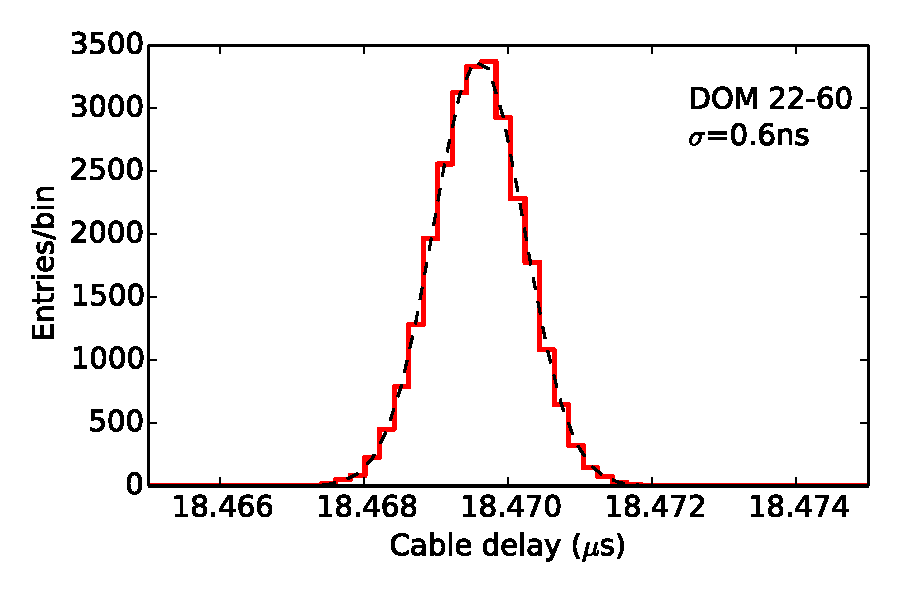
\includegraphics[width=0.6\textwidth]{graphics/dom/rapcal/tcal_hist_22-60.pdf}
 \caption{Distribution of one-way cable delays from multiple RAPCal
   measurements on DOM 22-60 (bottom of string 22).}
 \label{fig:rapcal_cable_len}
\end{figure}

The time calibration through the entire data aquisition and software
processing chain is verified using the LED flashers. During
commissioning, all 12~LEDs on each DOM are flashed simultaneously at
maximum brightness and the arrival timea of the first photons at the DOM above the flashing DOM
are recorded. Given the vertical spacing of 17~m on a standard IceCube
string and the group index of
refraction of  1.356 in ice at 400~nm, the expected light travel time
from the flashing DOM to the DOM above is 77~ns. In DeepCore, the DOM
vertical spacings are 10~m and 7~m, corresponding to light travel
times of 45~ns and 32~ns respectively. The mean light travel
time to the DOM above for all flashing DOMs in ice is shown in
Figure~\ref{fig:flashertiming}. The mean arrival time agrees with the
expectation for the DeepCore DOMs. For the standard DOMs, the oberved
light travel time is about 3~ns longer than the expected light travel
time, due to the effects of scattering in the ice over the longer distance. Muons are also used to
verify the time calibration, including the absolute time difference
between the IceTop surface stations and the in ice DOMs~\cite{IC3:perf}.

\begin{figure}[!h]
  \captionsetup[subfigure]{labelformat=empty}
  \centering
  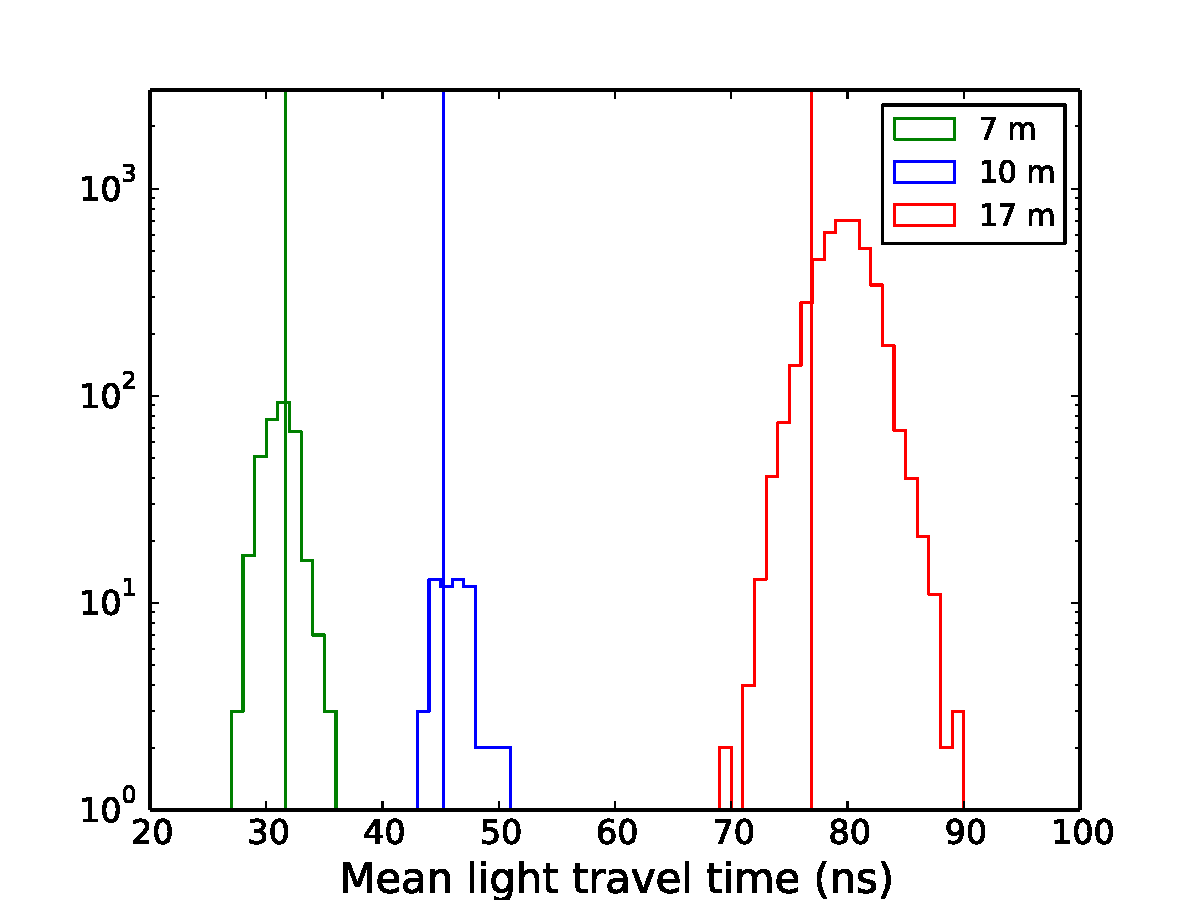
\includegraphics[width=0.8\textwidth]{graphics/dom/rapcal/flashmean.pdf}
  \caption{Time from flasher to DOM above for 17~m vertical spacing
    (red), 10~m vertical spacing (blue) and 7~m vertical spacing
    (green). The expected light travel time in ice for each distance is marked with
    vertical lines.}
  \label{fig:flashertiming}
\end{figure}

\subsubsection{\label{sec:domeff} DOM Optical Efficiency}

A baseline value for the photon detection efficiency was established
by combining PMT measurements at 337~nm and a separate model of
wavelength- and angle-dependent effects.  Absolute sensitivity
measurements were performed on 13 IceCube PMTs, using photons that
were Rayleigh scattered by 90$^{\circ}$  from a primary 337~nm laser
beam of known intensity~\cite{ICECUBE:PMT}. The results agreed well
with independent Hamamatsu measurements of sensitivity in the range
270~nm - 730~nm, which were then normalized to the 33~7nm measurement.  The resulting quantum efficiency at the center of the PMT and at 390~nm is 25\%.  A full simulation model for the DOM includes the wavelength dependence of the PMT response, optical absorption in the DOM glass and gel, discriminator threshold effects and photocathode nonuniformity.   The angle dependence is dominated by the shape of the photocathode and its response variation away from the center, which was measured for 135 PMTs~\cite{ICECUBE:PMT}.   

The laboratory-based efficiency model was supplemented with \textit{in situ} measurements using Cherenkov light from muons in the ice.  In one study, low energy muons (median energy 82~GeV) with well understood light emission were selected to illuminate the downward-facing PMTs in the ice as directly as possible. The numbers of photons detected at different distances from these muons were then compared to predictions of the simulation model~\cite{IC3:ereco}.  Based on this and other \textit{in situ}  analysis, the central value for the efficiency was adjusted upward by 10\% in the simulation, compared to the baseline.  For physics analysis, DOM efficiency is generally included as a nuisance parameter with prior uncertainty of 10\%,  which includes other uncertainties related to generation and propagation of the light. Additional laboratory measurements on assembled DOMs are in progress, including wavelength and angle dependent effects, and are expected to reduce uncertainties~\cite{ICECUBE:DOMEFF}.

The absolute calibration at 33~7nm was performed at room temperature
on a small subset of IceCube PMTs. The relative efficiency of all
assembled DOMs was separately measured as part of production testing,
using a 405~nm pulsed laser and a system of fibers and diffusers to
illuminate DOMs evenly within 50$^{\circ}$ of the optical axis.  Using
this system, the relative efficiency of DeepCore DOMs (high quantum
efficiency type) was measured to be higher by a factor 1.39 compared
to standard IceCube DOMs, agreeing well with a specified value of
1.40. Further \textit{in situ}  studies using muons yielded a factor of
1.35~\cite{ICECUBE:DC}, which is an effective value including the
Cherenkov spectrum folded with the different wavelength sensitivity
curves of the two types of PMTs.  The production testing system also
established the efficiency change from room temperature to
-40$^{\circ}$~C is less than 1\% when gain is maintained at the design value of $10^7$.  

%\subsubsection{Flasher Calibrations}

\subsection{Performance and Reliability}

As the DOMs are not serviceable after deployment, an extensive testing
protocol including temperature-cycling and cold-soaking ensured that bad
modules and early component failures were identified before shipping.
All DOMs were also re-tested at the South Pole before final deployment, to
screen out any modules damaged during transit.

As of 2016, 5397 of the 5484 deployed DOMs ($98.4\%$) are operating in
data-taking mode in the data acquisition system (see Table
\ref{tab:dom_failures}).  We classify DOM 
failures into two broad categories: failures during deployment and
freeze-in, and failures during subsequent operation.  The majority of the
failures (55) occurred before post-deployment commissioning; we hypothesize
that these are primarily attributable to cable failures, water leaks,
or freeze-in damage. 32 DOMs have failed after commissioning, and
we include in this count modules on a wire pair taken out of service when
the partner DOM on the same pair failed.  No particular pattern in the
failures is observed, other than they are typically during non-standard
operation or an exceptional event: a power outage, calibration run, or
flash filesystem upgrade.  The most recent two DOMs failed on May 23, 2013,
losing communications after a power outage.  Diagnosis of DOM failures
beyond identifying electrical shorts is challenging.

A number of DOMs have developed issues that affect their data-taking
configuration but are still usable.  The local coincidence settings of DOMs of
functional DOMs adjacent on a string to dead DOMs must also be
modified. These are enumerated in Table \ref{tab:dom_failures}.  

\begin{table}[h]
  \centering
  \begin{tabular}{| r | c |}
    \hline
    \bf{DOM failures} & \bf{87} \\
    \hline    
    deployment / freeze-in & 55 \\
    post-commissioning & 32 \\
    \hline
    \hline
    \bf{DOMs in Non-standard Mode} & \bf{171} \\
    \hline
    bad digitizer & 12 \\
    reduced PMT gain & 1 \\
    non-standard local coincidence & 158 \\
    \hline    
  \end{tabular}
  \caption{Number of DOM failures during deployment/freeze-in and after
    commissioning during detector operation, as well as DOMs with various
    issues (including a failed neighbor) causing them to be operated in a
    non-standard data-taking mode.} 
  \label{tab:dom_failures}
\end{table}

We can estimate the surviving fraction of DOMs 25 years after the original
deployment, assuming a constant, random failure rate after freeze-in.
Specifically, we calculate the Wilson score binomial confidence interval of
survival probability using the post-commissioning failure rate of DOMs
\cite{Wilson_Score}.  The estimated survival fraction as a function of
time is shown in Fig.~\ref{fig:dom_survival}; currently we estimate the
surviving fractEion in 2030 to be $97.3\pm0.3\%$.  While this simplified
model does not account for an increase in failure rate due to component aging, the
observed failure rate since detector completion of $2.0~\mathrm{yr}^{-1}$ is
significantly lower than the mean predicted rate of $4.5~\mathrm{yr}^{-1}$.  We attribute
this to infant mortality and/or to improved operational protocols that
minimize the number of DOM power cycles.

\begin{figure}[!h]
 \centering
 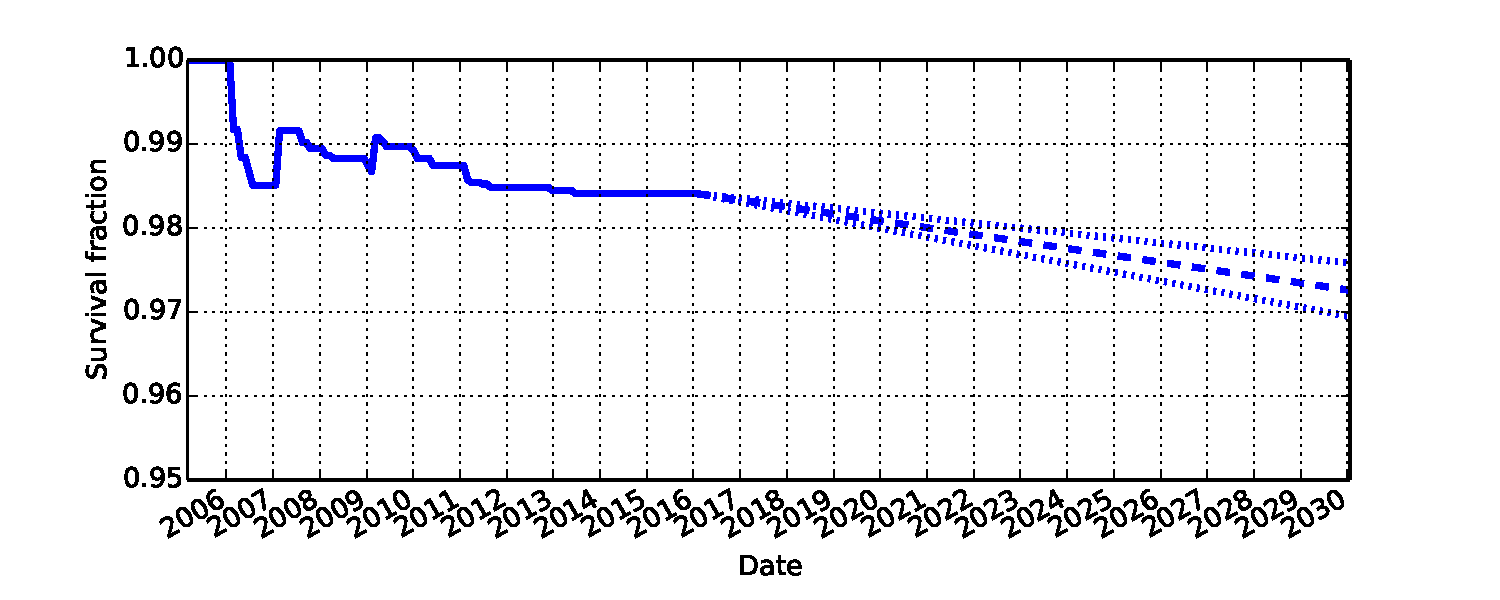
\includegraphics[width=0.95\textwidth]{graphics/dom/reliability/dom_survival.pdf}
 \caption{Actual and predicted fraction of surviving DOMs versus time, based on an assumed
 constant post-freeze-in failure rate.  The dotted lines indicate the
 central and 95\% CL estimates.  Increases before 2011 are due
 to deployments of new strings.} 
 \label{fig:dom_survival}
\end{figure}

%We have over $N$ DOM years in ice.  What can be said about 
%the reliability?  This section could be quite important.

\subsubsection{Baseline Stability}

The beacon hits from which the digitizer baselines are derived are
monitored continuously throughout the year. The average value of the
beacon baselines are very stable, with shifts of no more than
0.2~counts year to year, which corresponds to 0.018~mV in the FADC and
0.025~mV in the high gain ATWD channel. The single photoelectron
charge peak is stable to within 0.05~PE. The baseline shifts from May
2015 to April 2016 are shown in
Figure~\ref{fig:baseline_stability_2015}. 

\begin{figure}[!h]
 \centering
 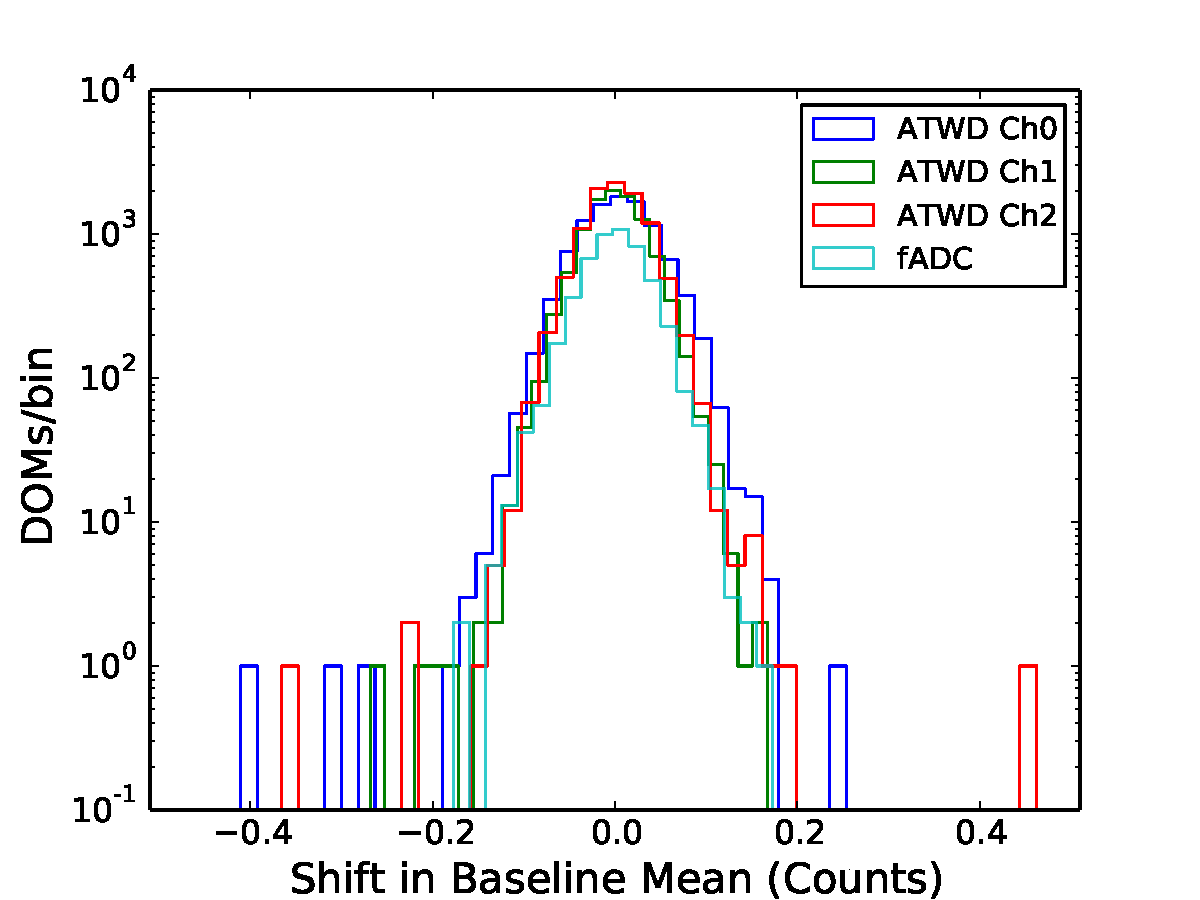
\includegraphics[width=0.6\textwidth]{graphics/dom/reliability/baseline_stability_2015.pdf}
 \caption{Distribution of shifts in baseline values in all ATWD
   channels and the FADC for all DOMs between May 2015 and April
   2016. The DOM configuration was unchanged during this period.}
 \label{fig:baseline_stability_2015}
\end{figure}

Every year when the detector
is recalibrated, adjustments in the SPE discriminator threshold can
cause shifts of up to 0.6~counts (0.54~mV) in the FADC
baselines. ATWD baselines are unaffected by the SPE discriminator
setting. Correcting recorded waveforms for the effect of transformer
coupling as described in Sec.~\ref{sec:waveformcal} has
the side effect that small DC offset errors are converted into
apparent PMT current that increases linearly in time over the course
of a few microseconds. The effect is stronger for DOMs with old
type toroid transformers, where a baseline error of 0.6~counts can
turn an actual deposited charge of 1~PE into a measured charge of over
2~PE with an unphysical time structure. The observed distortion in a
simulated single photoelectron charge due to FADC baseline shifts is
shown in Figure~\ref{fig:charge_fadcshift}  Therefore, whenever the
discriminator thresholds are changed, the FADC baselines are measured
again and the values used for calibration are refreshed. As long as
the discriminator thresholds are unchanged, the baselines are stable
to within 0.2~counts
as shown above, and no charge distortion is seen at that level of
baseline stability.

\begin{figure}[!h]
 \centering
 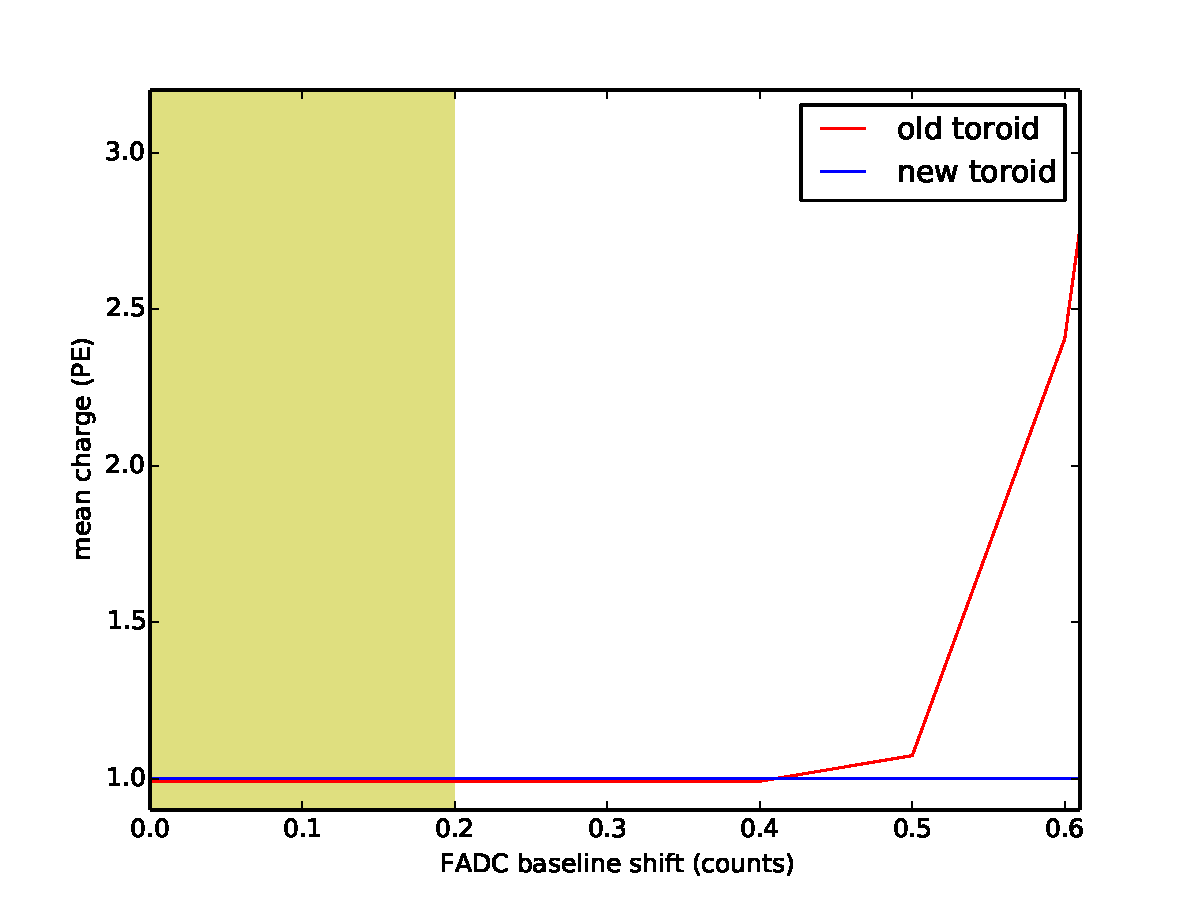
\includegraphics[width=0.8\textwidth]{graphics/dom/reliability/charge_fadcshift.pdf}
 \caption{Reconstructed charge from a simulated single photoelectron
   deposit as a function of FADC baseline shift, for both old and new
   toroid DOMs. The shaded region indicates the observed range of
   baseline variation from the nominal value in ice; no observable
   distortion in the charge spectrum is seen at these values.}
 \label{fig:charge_fadcshift}
\end{figure}

The baselines are sensitive to radio frequency interference (RFI). In
2009, RF signals from a radar transmitter broadcasting at 46.3~MHz
appeared as sinusoidal or spiky signatures in the waveform
baselines. Also in 2009, a DOM 68-42 ``Krabba'' was damaged by a too-high
voltage setting during DOM calibration, and appeared to begin
sparking, causing sinusoidal waveforms to appear in the baselines of
neighboring DOMs.
%more figures go here: waveforms from Krabba disaster and Meteor radar

\subsubsection{Gain Stability}

The gain stability of the DOM, or the stability of the amplified charge
from converted photons, depends on a number of factors including stability
of the PMT high voltage, Main Board channel amplifiers, and the digitizers.
We can examine these subsystems using both historical calibration results
as well as by tracking the SPE charge during data-taking.

The electronic gain stability of the DOM includes variations in the
front-end electronic amplifiers and the digitizers themselves.  The
stability is checked by comparing the Main Board channel amplifier gains
from sets of calibrations taken from 2011 to 2016 (see
Fig.~\ref{fig:domcal_ch_gain}).  From year to year, the amplifier gain
calibration is repeatable to 0.1\%, 0.2\%, and 0.5\% in the high-gain,
medium-gain, and low-gain channels respectively.  Since detector completion
in 2011, a small systematic shift of $-0.3\%$ is visible in the low-gain
channel, but this is corrected by updating the calibration constants of
each DOM.

% JK: DOMCal History.ipynb
\begin{figure}[!h]
  \captionsetup[subfigure]{labelformat=empty}
  \centering
  \subfloat[]{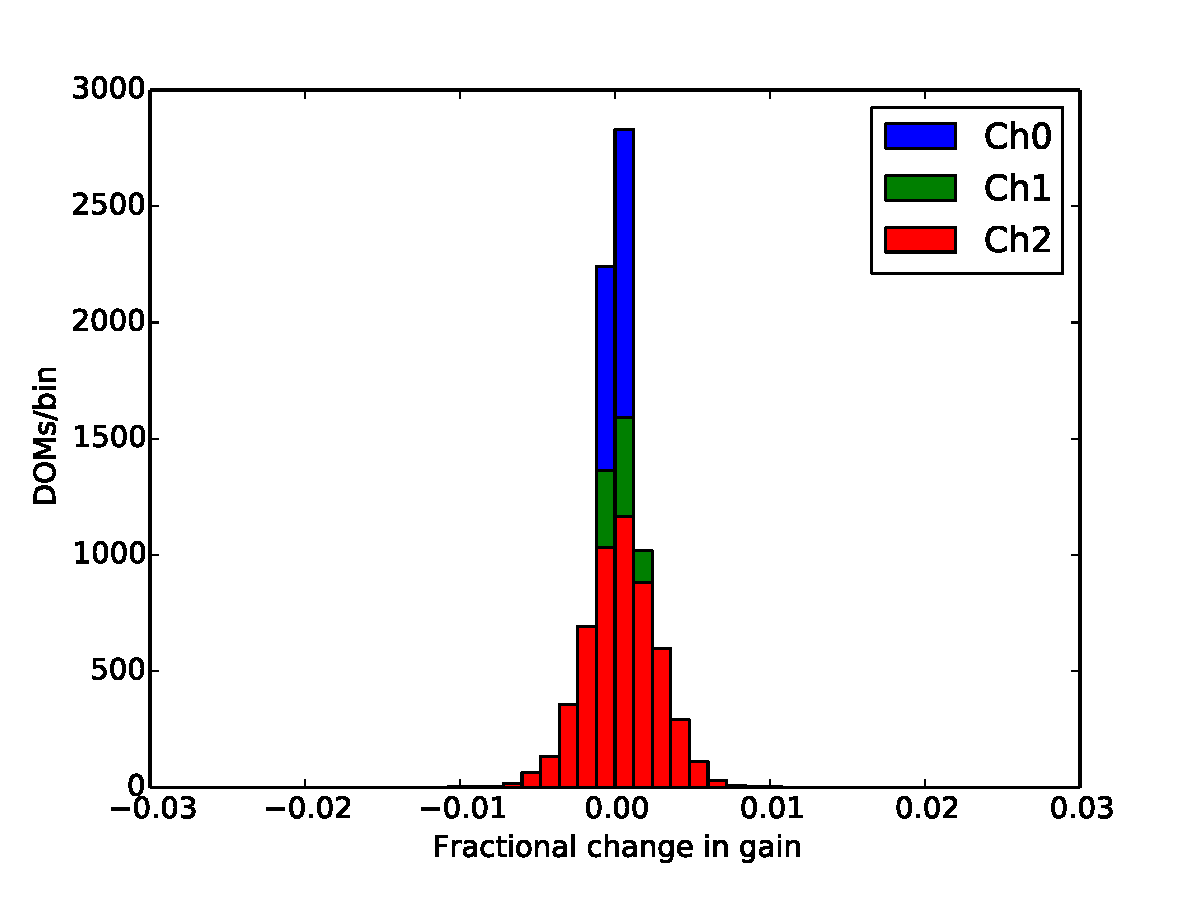
\includegraphics[width=0.5\textwidth]{graphics/dom/reliability/channel_gain_shift_2016_2015.pdf}}
  \subfloat[]{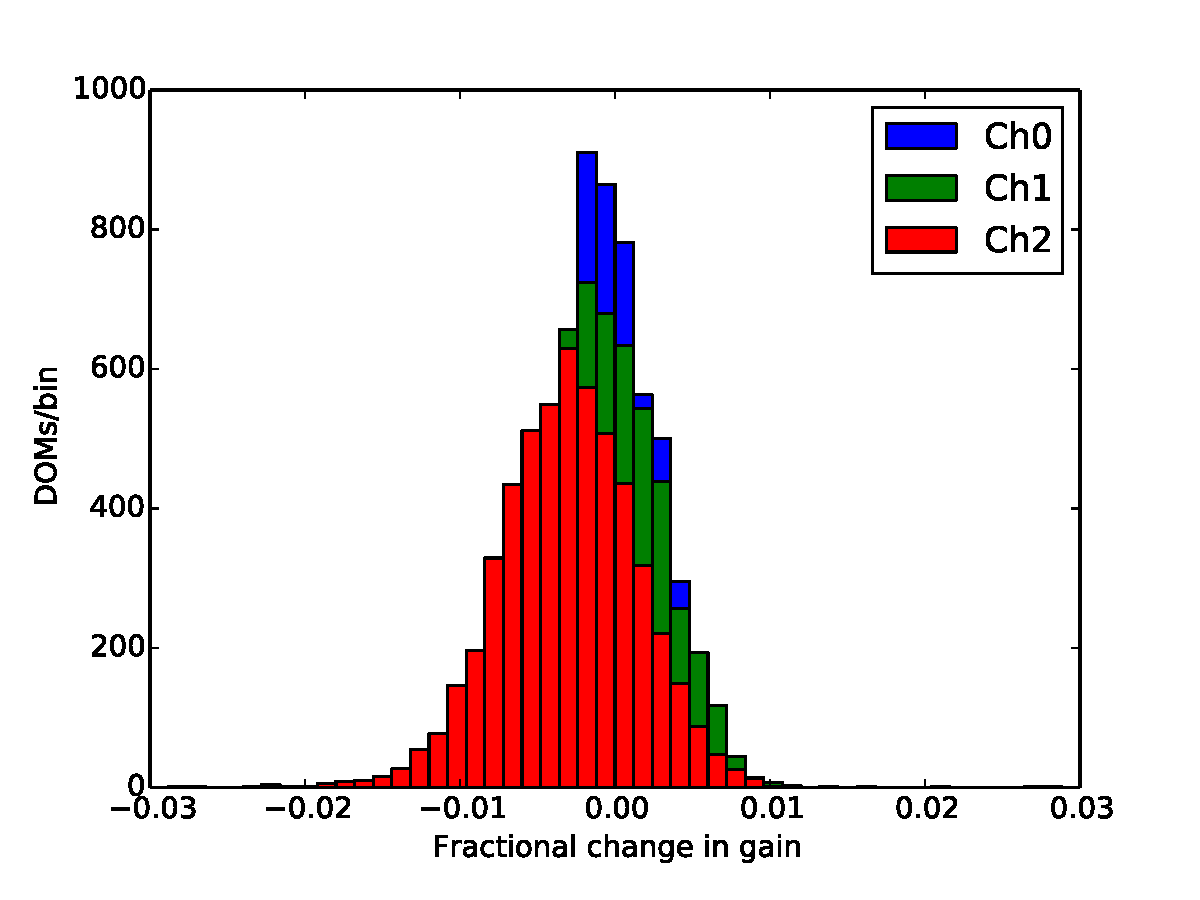
\includegraphics[width=0.5\textwidth]{graphics/dom/reliability/channel_gain_shift_2016_2011.pdf}}
  \caption{Fractional DOM channel amplifier gain shifts, from 2015 to
    2016 (left) and 2011 to 2016 (right).  Channels 0, 1, and 2 are
    high-gain, medium-gain, and low-gain respectively.}
  \label{fig:domcal_ch_gain}
\end{figure}

The PMT gain stability is monitored during data-taking using the
single photoelectron peak of the charge distribution on each DOM due
to cosmic ray muons. A
Gaussian + exponential function is fit to the peak region as in Figure~\ref{fig:spe_fit_thresh} and the mean of the Gaussian is
tracked throughout the year. The threshold, defined as the point which
contains 1\% of the charge in the histogram, is also tracked through
the year. The peak position is calibrated to 1~PE
and is stable to within 0.01~PE for 95\% of all DOMs as shown in
Figure~\ref{fig:gain_spe_stability}. Over 99\% of DOMs show no
measurable change in the threshold as long as the discriminator
thresholds are unchanged; these settings are only changed once per year.

\begin{figure}[!h]
 \centering
 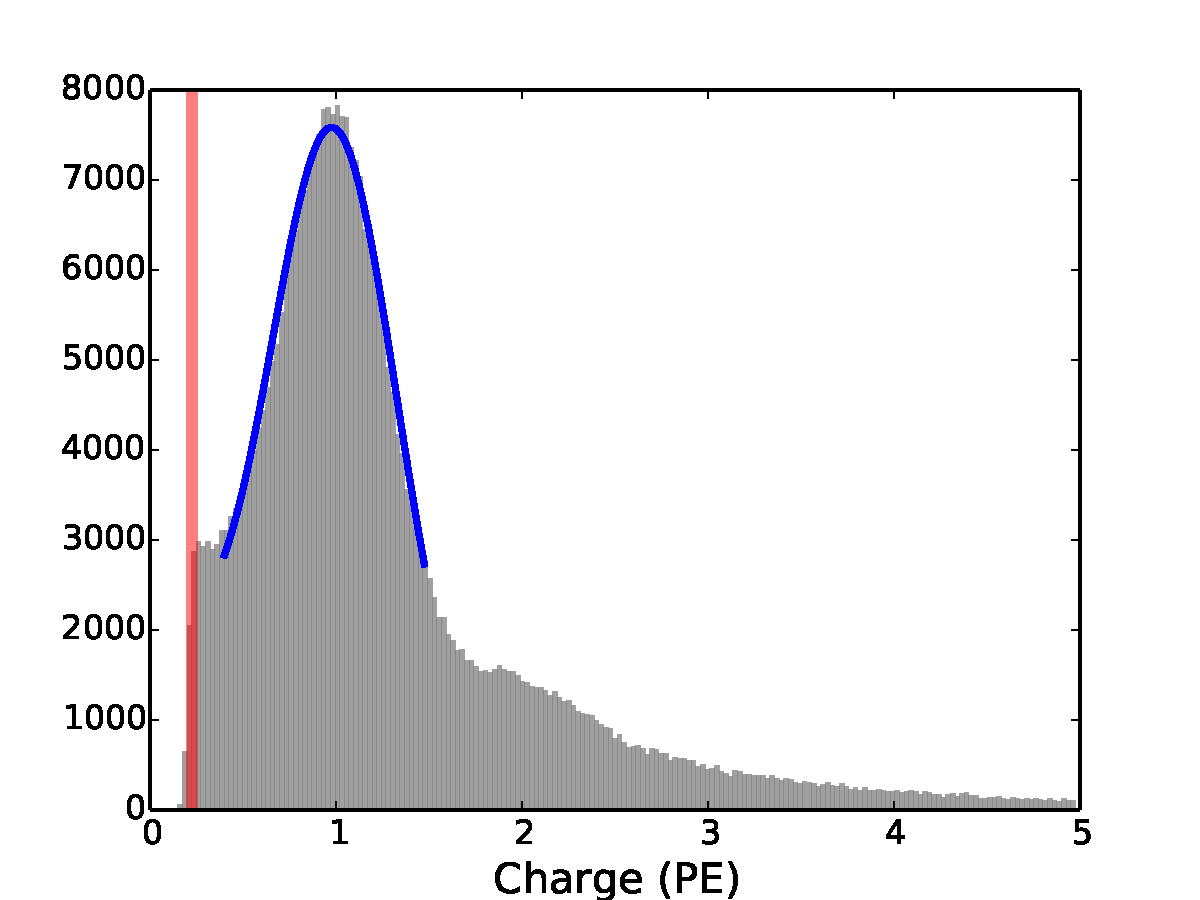
\includegraphics[width=0.6\textwidth]{graphics/dom/reliability/chargedist.pdf}
 \caption{Charge distribution on a typical in-ice DOM. The threshold
   is marked in red and a gaussian + exponential fit to
   the SPE region is shown in blue. The mean of the gaussian is used
   to monitor the gain stability.}
 \label{fig:spe_fit_thresh}
\end{figure}

\begin{figure}[!h]
  \captionsetup[subfigure]{labelformat=empty}
  \centering
  \subfloat[]{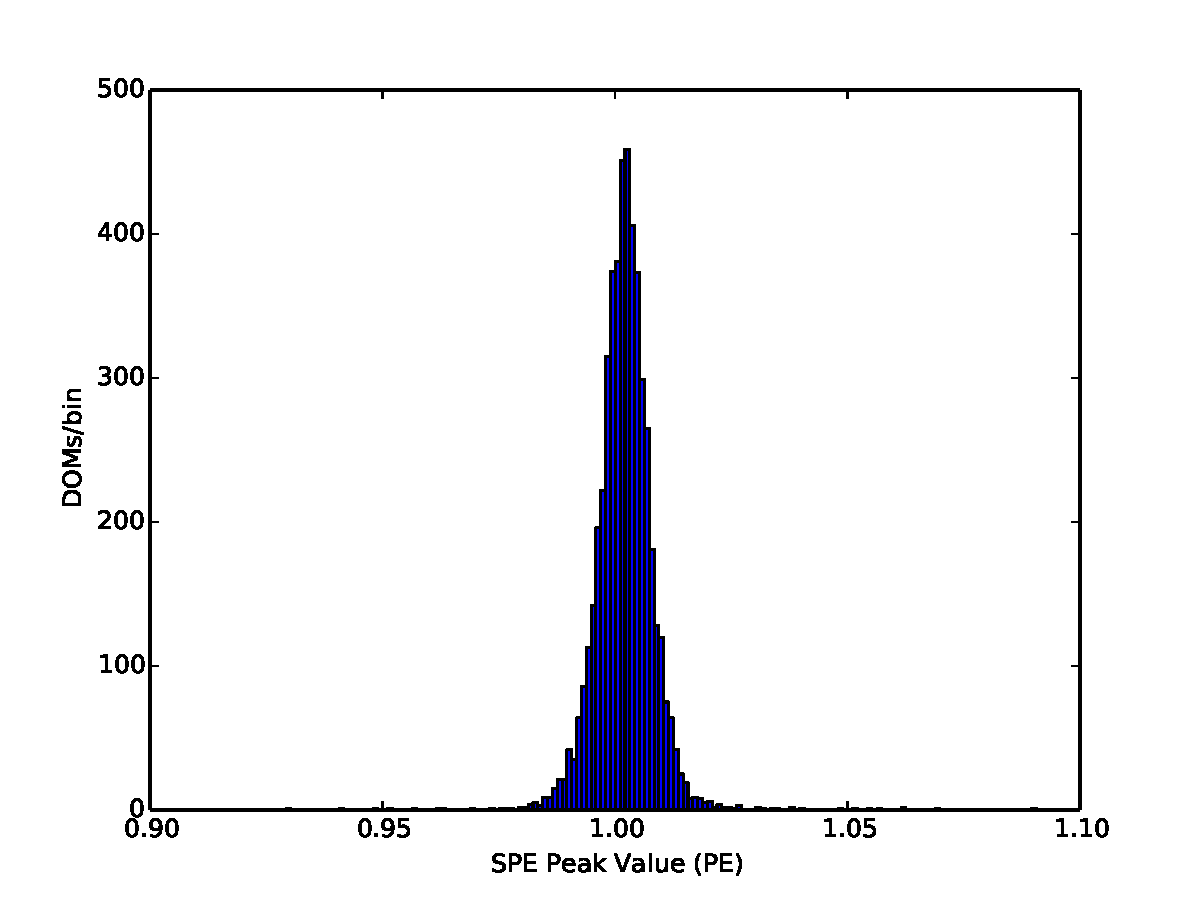
\includegraphics[width=0.5\textwidth]{graphics/dom/reliability/mean_value_2015.pdf}}
  \subfloat[]{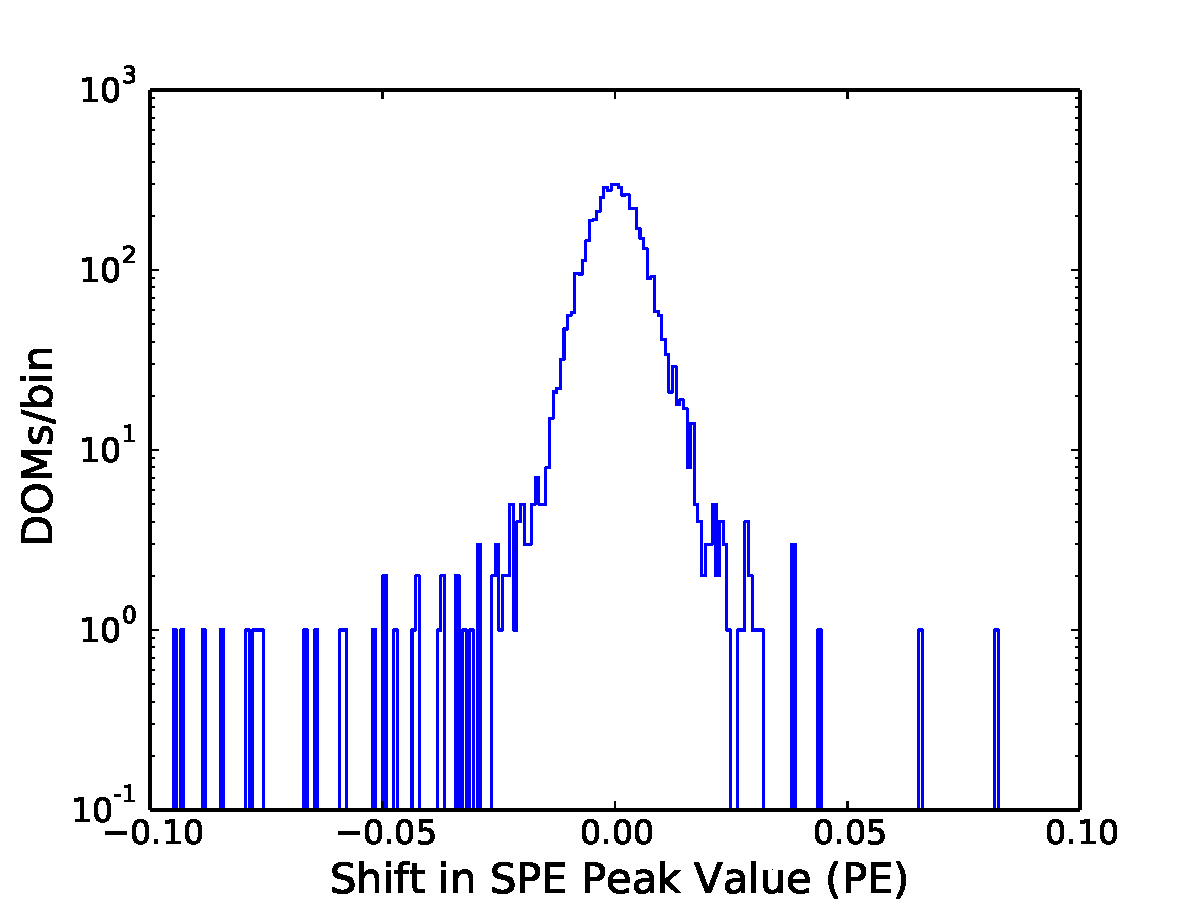
\includegraphics[width=0.5\textwidth]{graphics/dom/reliability/meandiff_2015.pdf}}
  \caption{Distribution of the mean of the Gaussian fit to the SPE
    peak (left) and the shift in this value in every in-ice DOM between  May 2015 and April
   2016.}
  \label{fig:gain_spe_stability}
\end{figure} 

There are on the
order of 12~DOMs which show unpredictable, abrupt shifts in the SPE peak
position of 0.05~PE or more. Figure~\ref{fig:gainshift_spe} shows the time history of the
SPE peak position of one of these DOMs over 4~months. The peak shift
corresponds to increases or decreases in the MPE scaler rate,
indicating that the SPE peak shift is indeed caused by a change in the DOM
gain. However, the SPE scaler rate is stable, indicating that the
probability to detect single photons is unchanged.

\begin{figure}[!h]
 \centering
 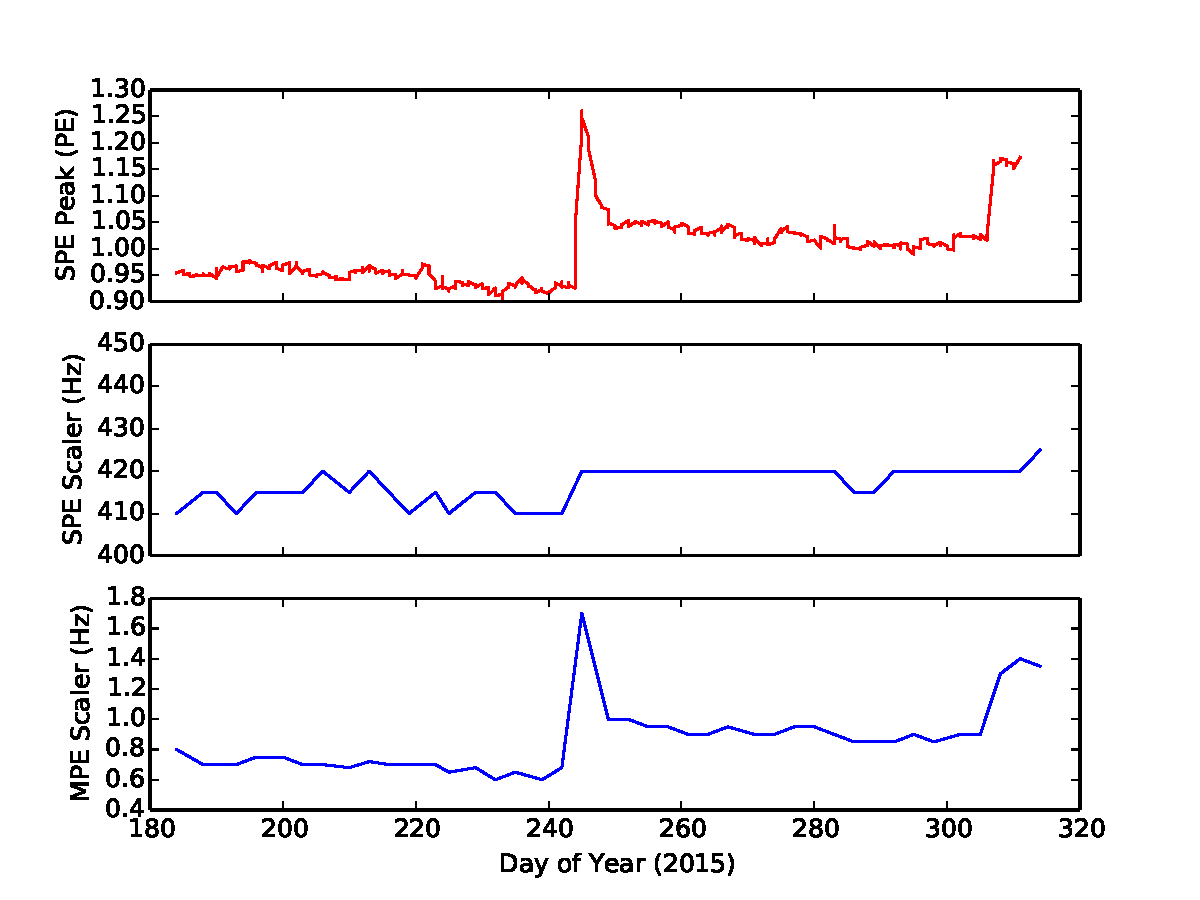
\includegraphics[width=0.8\textwidth]{graphics/dom/reliability/gainshift.pdf}
 \caption{Mean of the Gaussian fit to the SPE peak (top) and the SPE
   scaler rate (middle) and MPE
   scaler rate (bottom) from July 2015 to November 2015 for a DOM
   which shows unpredictable gain shift behavior. The DOM
   configuration was unchanged during this period.}
 \label{fig:gainshift_spe}
\end{figure}

\subsubsection{Optical Sensitivity Stability}

The detector response in IceCube is calibrated with low energy muons as
described in \cite{IC3:ereco}. The detector response is monitored in each run using the track
detection probability (TDP) calculated from high
multiplicity muon tracks with more than 30 hits in IceCube. The muon
tracks are reconstructed using the likelihood methods described in
\cite{IC3:ereco}; charge and time information from the DOM under study excluded
from the reconstruction. The TDP is
defined for each DOM as the ratio of the number of detected tracks
within 100~m of the DOM to the total number of tracks within 100~m of
the DOM. This ratio depends both on the optical properties of the ice
near the DOM and the optical efficiency of the DOM. We do not attempt
to separate
these effects in the TDP, but rather use the TDP to monitor the
overall stability of the detector response. Figure~\ref{fig:tdp} shows the TDP on
string 80, which includes both standard and HQE DOMs; the TDP is
20\% - 25\% higher for HQE DOMs than for neighboring standard
DOMs, whereas the quantum efficiency is 35\% higher. The TDP is stable to within 1\% since 2012, when the baselines
were stabilized by being set in the DAQ configuration. Figure~\ref{fig:tdp} shows
the difference in the TDP for all DOMs between a run in 2012 and a run
in 2015.
%Figure goes here: TDP on string 80, showing the jump in DOMs 30-43
%which are HQE
%Figure goes here: TDP difference between 2012 run (after April 29)
%and 2015 run.

\begin{figure}[!h]
  \captionsetup[subfigure]{labelformat=empty}
  \centering
  \subfloat[]{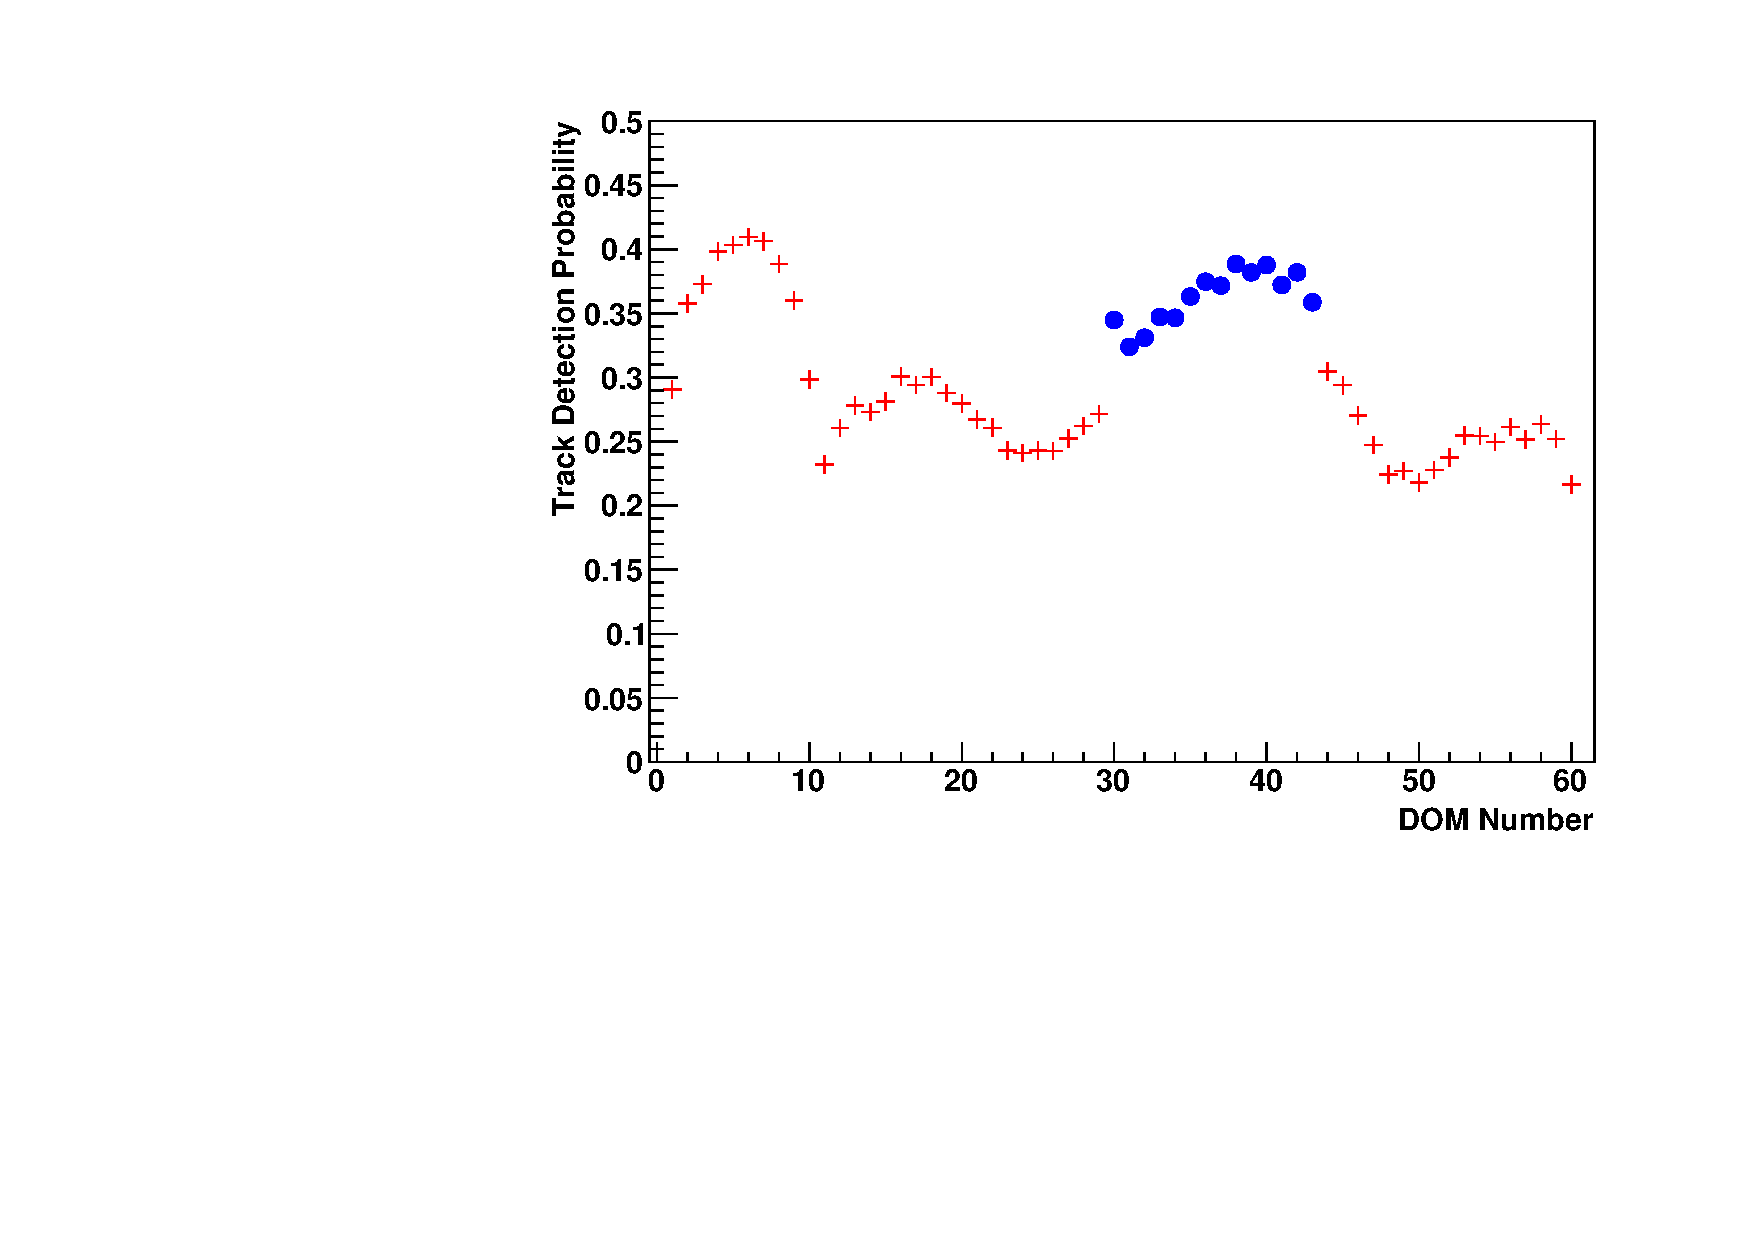
\includegraphics[width=0.5\textwidth]{graphics/dom/reliability/tdp_onestring.pdf}}
  \subfloat[]{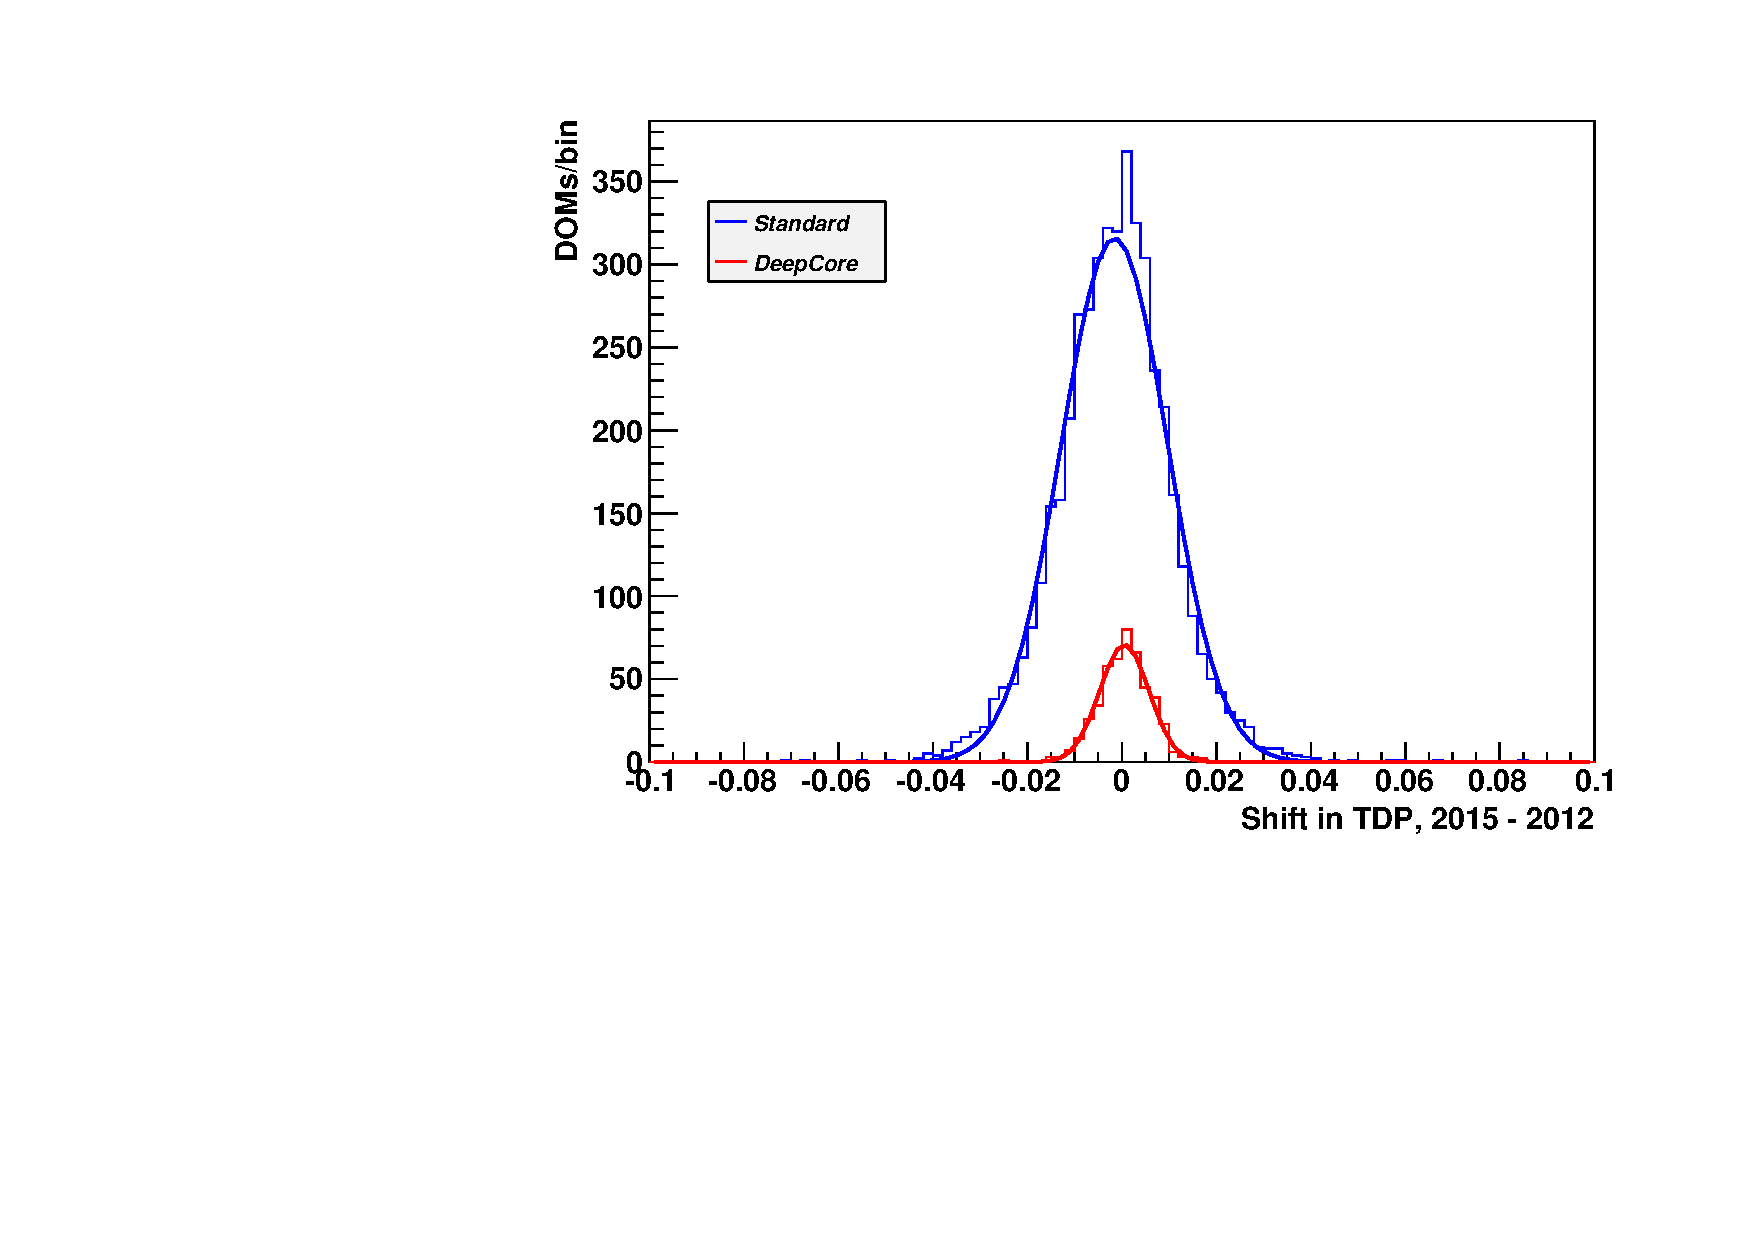
\includegraphics[width=0.5\textwidth]{graphics/dom/reliability/tdpcomparison.pdf}}
  \caption{Left: Track detection probability in string 80, with a
    mixture of standard DOMs (red crosses) and HQE DOMs (blue
    circles). Right: Shift in track detection probability for all in
    ice DOMs between 2012 and 2015; standard DOMs are in blue and
    DeepCore DOMs are in red. The mean of the Gaussian fit to
    the TDP shift in the standard DOMs is -0.1\% and the means of the Gaussian fit to
    the TDP shift in the DeepCore DOMs is 0.05\%.}
  \label{fig:tdp}
\end{figure}

The detector response stability is also measured with the {\it in
  situ} light sources in IceCube. Both the in-ice calibration laser
\cite{IC3:SC} and the flasher LEDs show less than 1\% difference in the total
charge collected between 2012 and 2015. 

\subsubsection{\label{sect:darknoise}Dark Noise}


The vast majority of background hits result from dark noise, i.e. effects that lead to the emission of an electron from the cathode of the PMT in the absence of an external photon. The total hit rate of DOMs with normal quantum efficiency PMTs is on average \SI{560}{\hertz} and \SI{780}{\hertz} for high QE DOMs. 
The dark noise is composed of two major components. Electronics noise and radioactive decays in the material form the uncorrelated noise pulses of Poissonian nature with a rate between \SI{230}{\hertz} and \SI{250}{\hertz} that follows the Richardson law for thermal emission. 
The remaining component is the so-called correlated noise
with a hit rate that increases with decreasing temperature from \SI{280}{\hertz} to \SI{340}{\hertz} (Figure \ref{fig:dom_darknoise_vs_temperature}). 
This temperature dependent noise rate profile was acomplished by combining a measured temperture profile of the the South Pole ice cap \cite{price2002temperature} with a fit of the Poissonian expectation of the total dark noise rate to every individual DOM.

\begin{figure}
 \begin{minipage}[t]{0.45\linewidth}
 \centering
  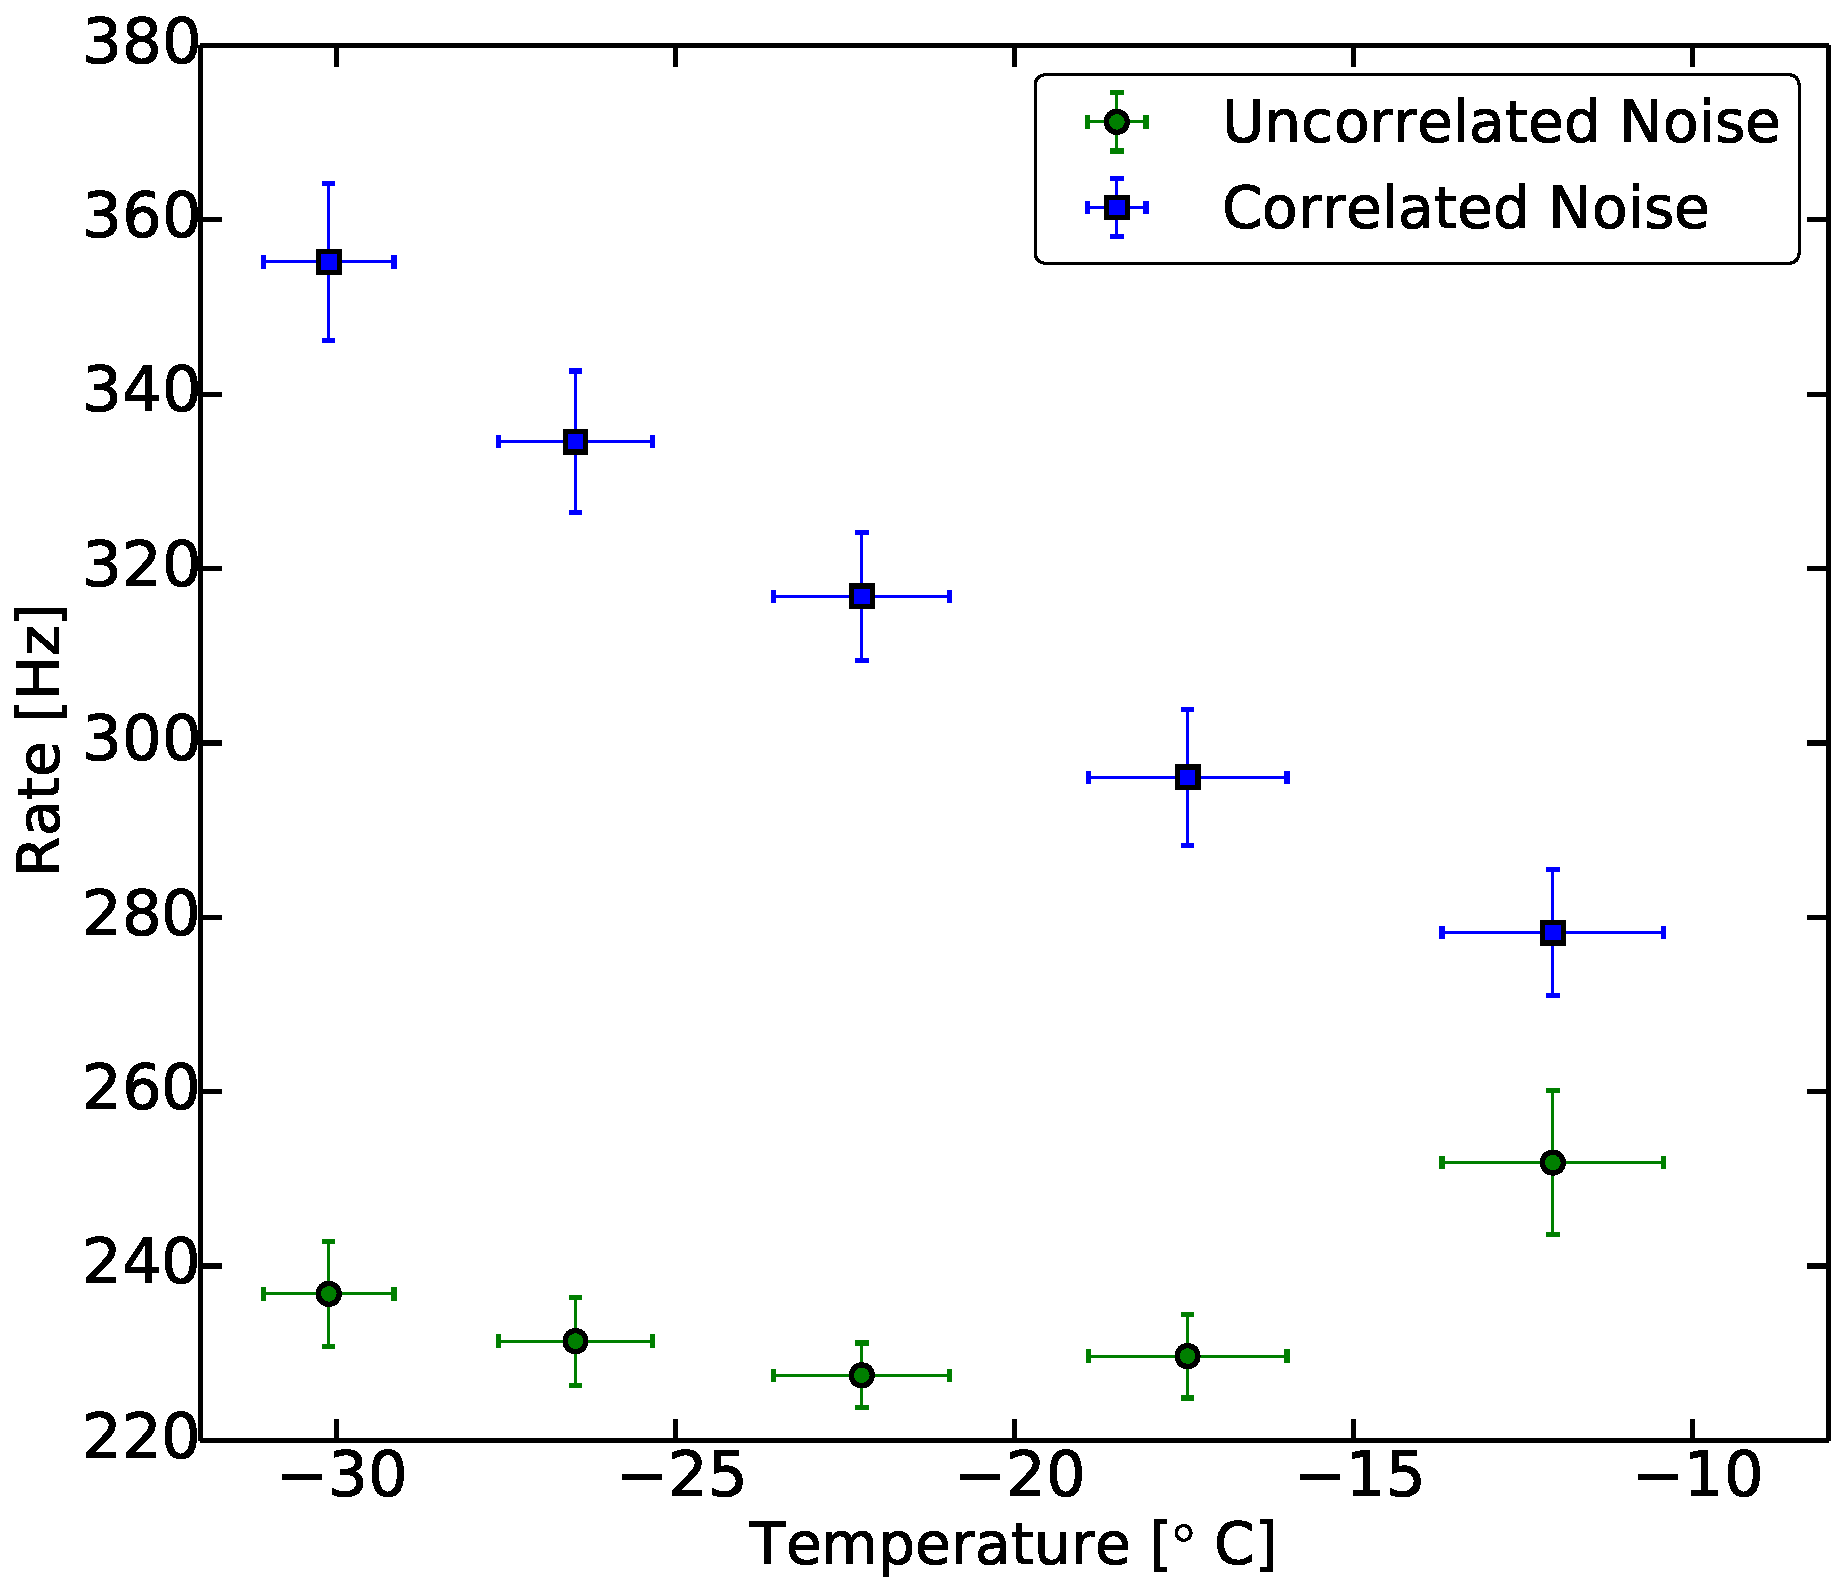
\includegraphics[width=\textwidth]{graphics/dom/performance/darknoise/HitRatevsTemp_inice_nomuons_nofit_bigfont.pdf}
 \caption{Dark noise rate in IceCube as a function of temperature, obtained from hitspooling
 data. Each data point represents the average of 12 DOM layers from 78 strings (DeepCore excluded)}
 \label{fig:dom_darknoise_vs_temperature}
 \end{minipage}
\hfill
 \begin{minipage}[t]{0.45\linewidth}
 \centering
  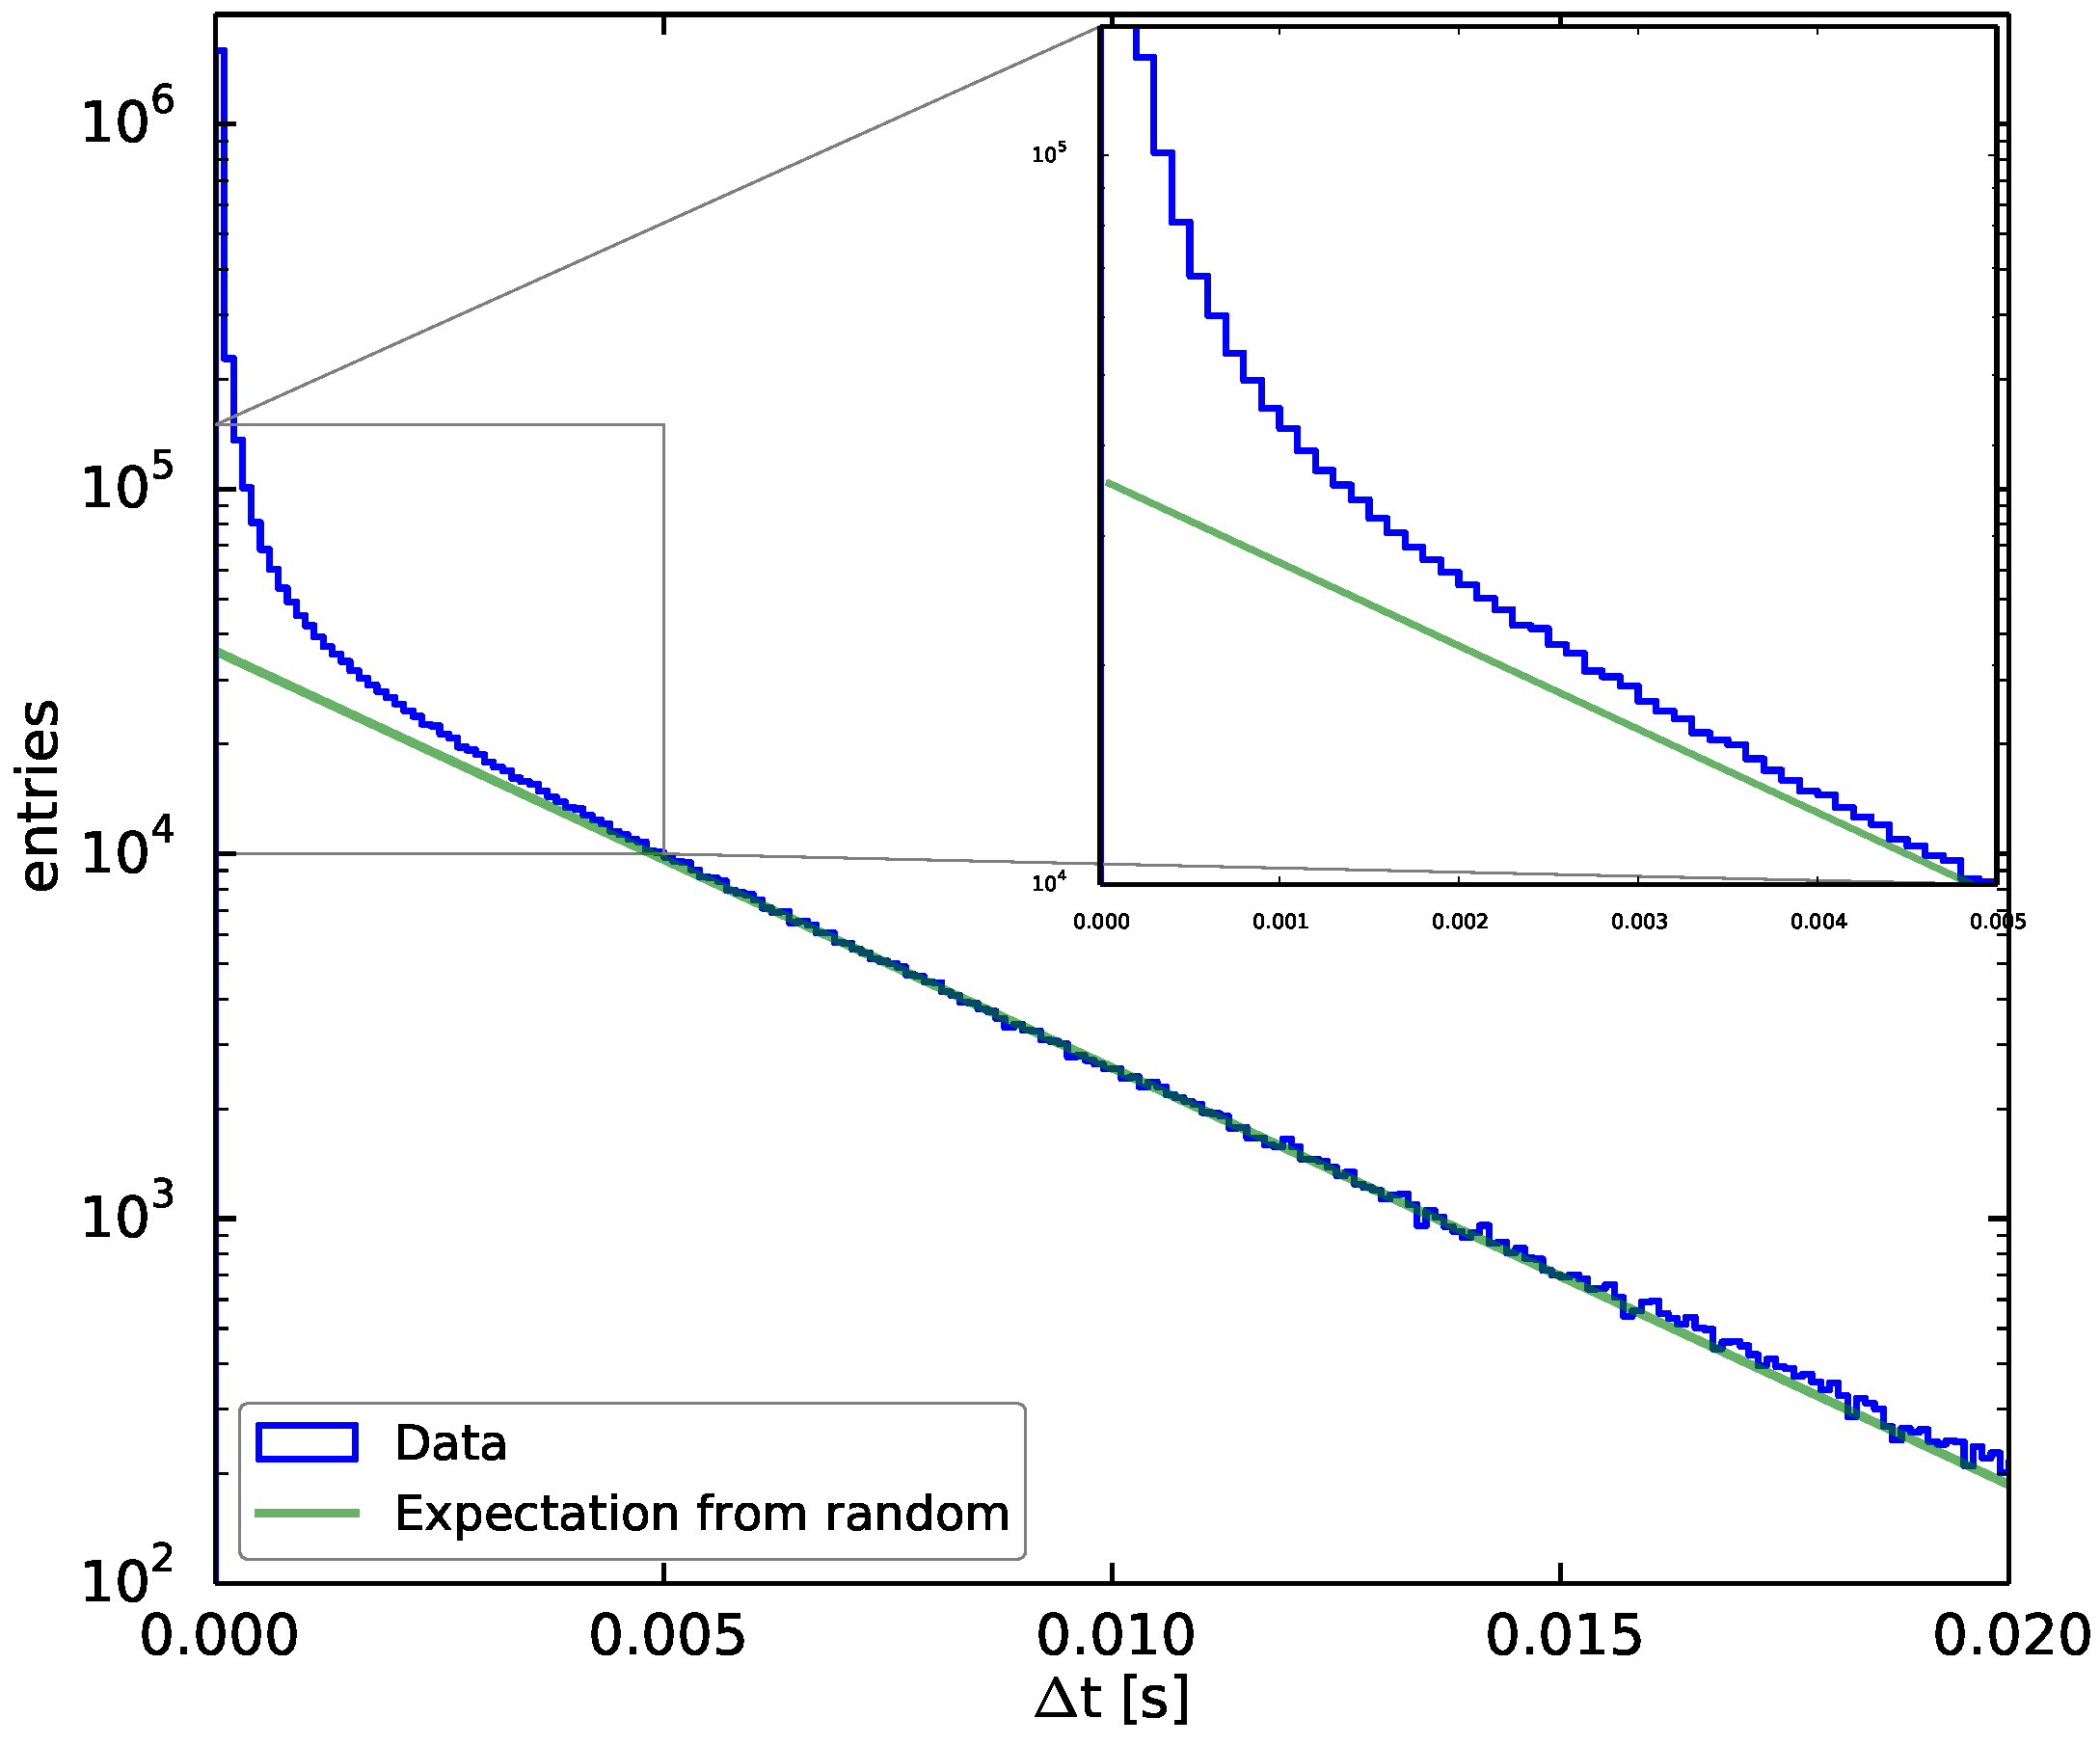
\includegraphics[width=\textwidth]{graphics/dom/performance/darknoise/DarkNoise_Layer2Doms.pdf}
 \caption{Time interval between successive hits for all next-to-top layer DOMs (DeepCore excluded).}
 \label{fig:darknoise_deltaT}
 \end{minipage}
\end{figure}

The correlated noise component manifests itself in an overabundance of short time intervals between hits in a single DOM compared to the expectation from random (Figure \ref{fig:darknoise_deltaT}). The short time intervals are correlated and clustered in bursts with an average number of hits per burst rising from \num{3.3} at \SI{-10}{\celsius} to \num{3.8} at \SI{-30}{\celsius}. A detailed study with hitspooling data shows that the phenomenology of the correlated noise component in IceCube is in general in good agreement with results reported in the literature with a satisfying physical explanation still to be determined. Best candidate for the source of the entire process is luminescence triggered by radioactive decay of elements like Thorium and Uranium in the glass of the DOM.
The various sources of dark noise present in a DOM are best visible when histogramming the time between subsequent raw data hits ( or hitspool data, see Section \ref{sec:domhub_hitspool}) in a DOM on a logarithmic scale, as shown in Figure \ref{fig:darknoise_deltaT_components}. An overview of the various noise components is also given in Table \ref{tab:noise}. The so far unmentioned afterpulses, a common feature of PMTs, is attributed to ionization
of residual gases by electrons that were accelerated in between the dynodes. 

IceCube uses the result of these noise studies to build a parametrized noise model that is needed for an accurate detector simulation \cite{larson2013simulation}.

\begin{table}[h!]
\caption{Characteristics of noise components in IceCube DOMs, adapted from \cite{stanisha_noise_14}.}
  \centering
  \footnotesize
\begin{tabularx}{\textwidth}{lXXX}
\toprule
Noise Component& Origin & Distribution & Parameters \\
\midrule
Afterpulses & PMT & Gaussian & $\mu = \SI{6}{\micro\second}$ \newline $\sigma = \SI{2}{\micro\second}$\\
Uncorrelated & Thermal noise\newline Radioactive Decay & Poissonian & $\lambda = \sim \SI{250}{\hertz}$\\
Correlated & Luminescence (?) & Log-normal & $\mu = \num{-6} [\log_{10}(\frac{\Delta T}{s})]$ \newline $\sigma = \num{0.85} [\log_{10}(\frac{\Delta T}{s})]$\\
\bottomrule
\end{tabularx}
\label{tab:noise}
\end{table}

\begin{figure}[!h]
 \centering
  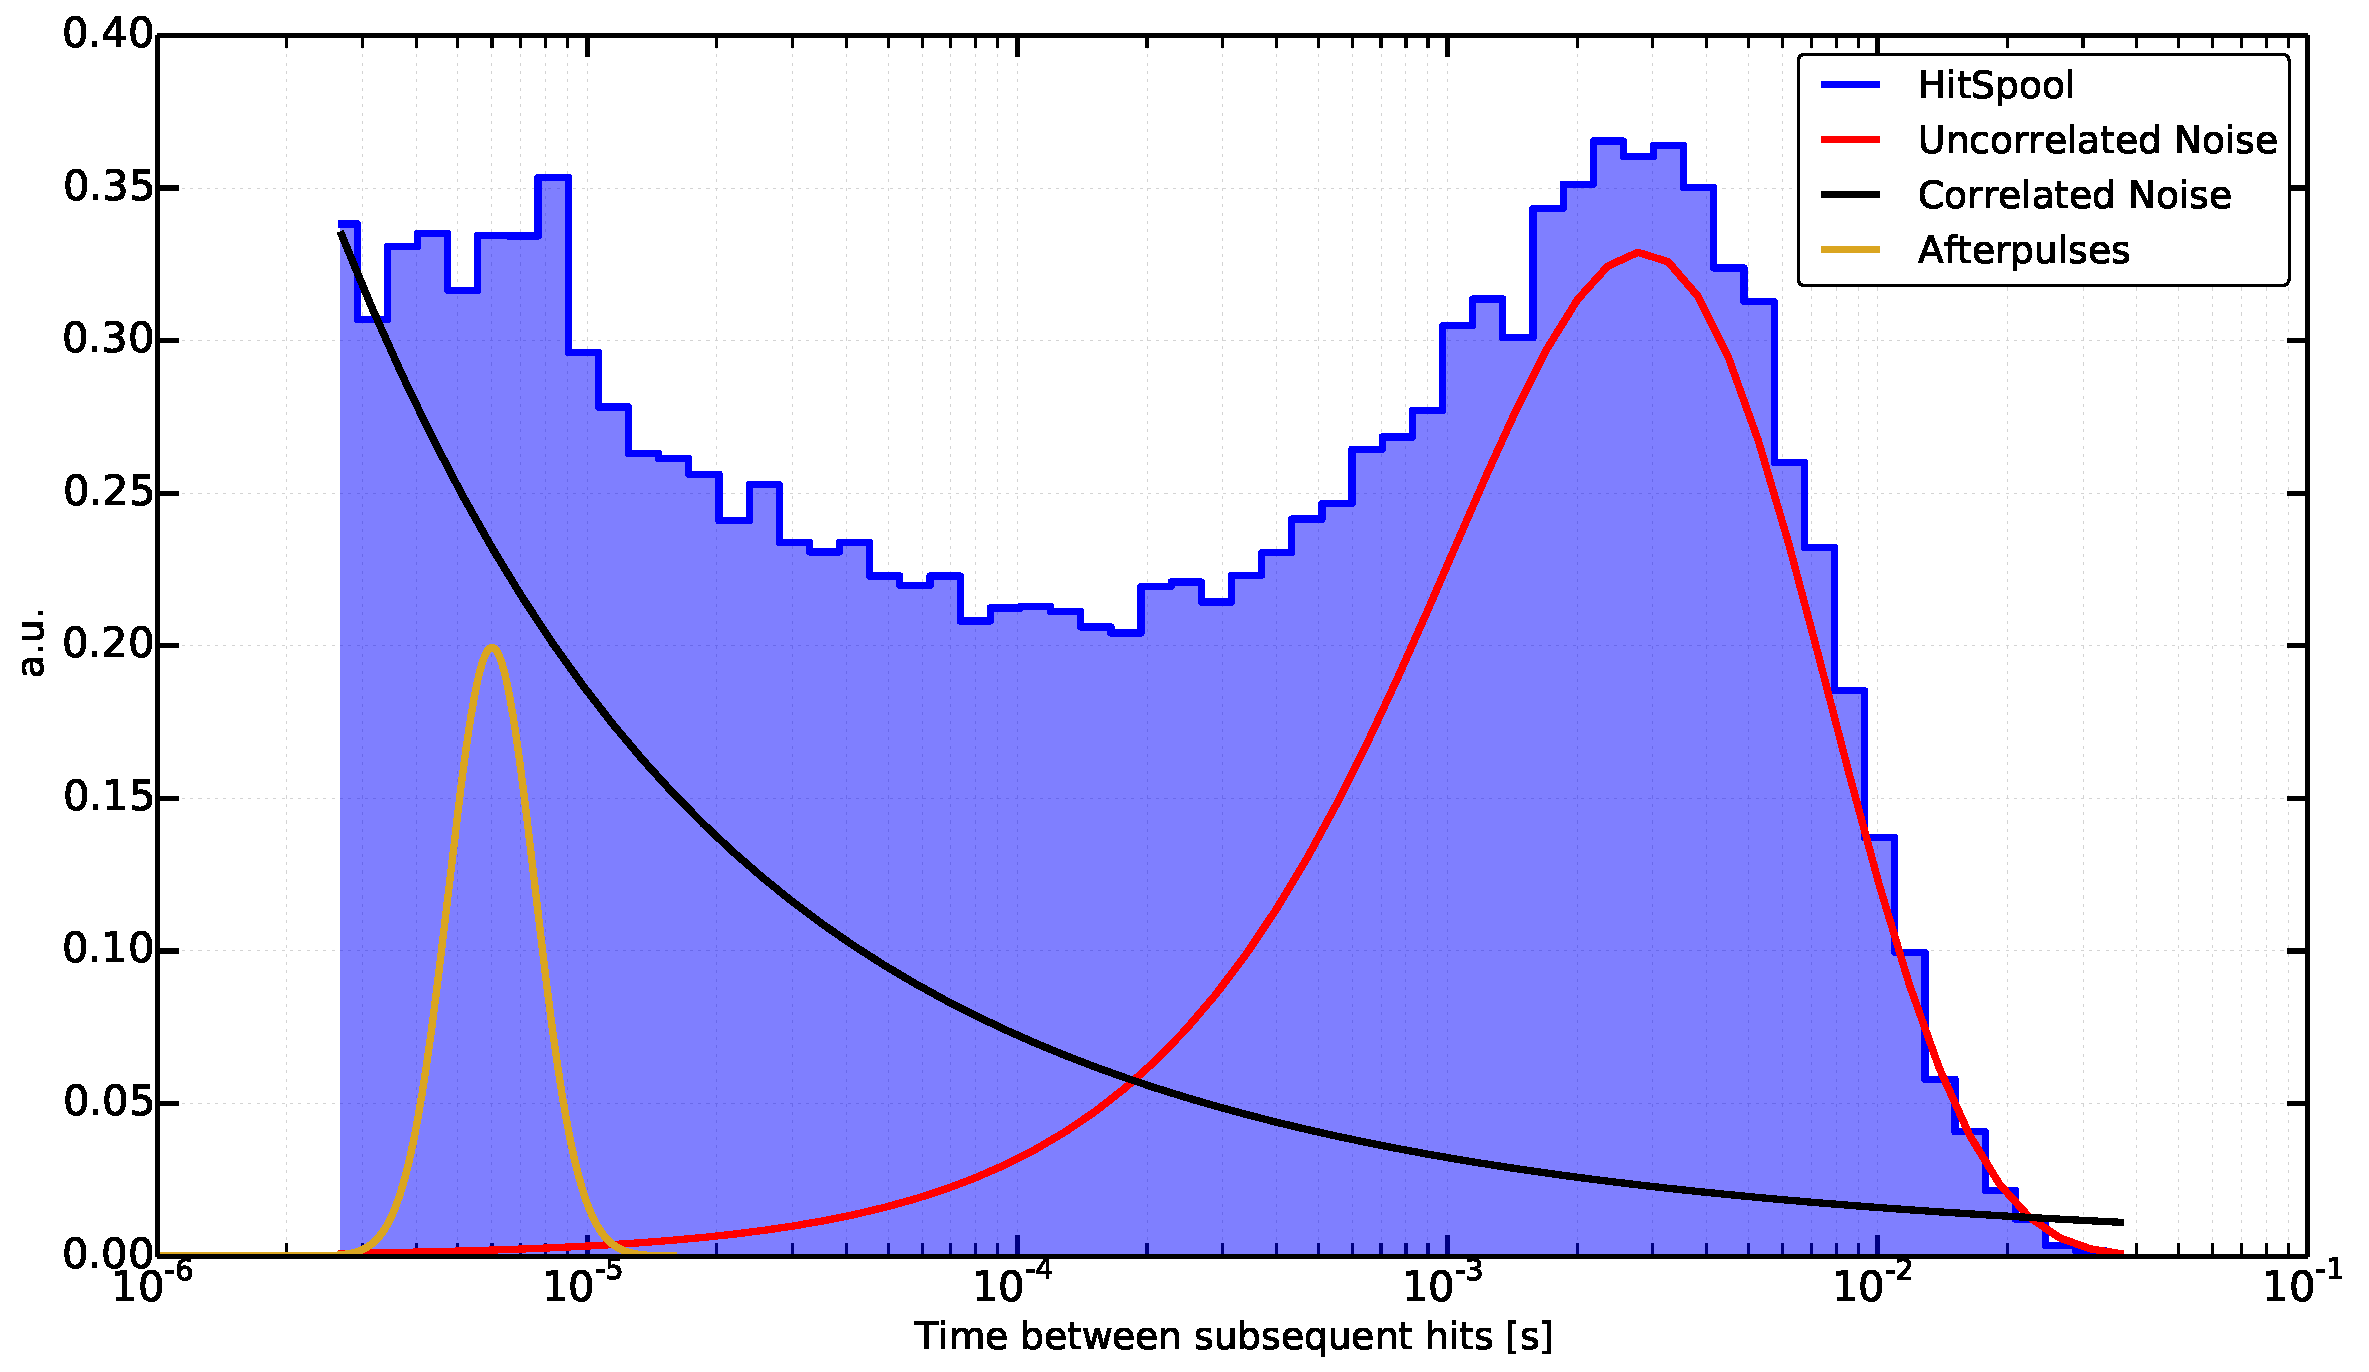
\includegraphics[width=0.8\textwidth]{graphics/dom/performance/darknoise/SingleDOM_HitSpool_Hits_deltaT_fits_example.pdf}
 \caption{Histogram of time differences between successive hits from HitSpool data of
DOM 15-27 (blue) on a logarithmic scale in order to visualize the different noise components
(without prepulses which are comparatively insignificant) \cite{heereman2015hitspooling}.}
 \label{fig:darknoise_deltaT_components}
\end{figure}


The evolution of the dark noise rate over time was investigated using data from the supernova scaler stream \cite{IC3:supernova, briedel_phd}. There is a exponential decay over the course of the data set which is caused by a decreasing triboluminescence in general arising from a `freeze-in` procedure of newly deployed DOMs. As the ice refreezes after deployment, it becomes cleaner and impurities introduced during the drill process (mainly trapped gas) are pushed inwards into a column nearly at the center of the drill hole. This mechanical stress requires breaking bonds in the ice which in turn can lead to triboluminescence. This effect is studied preferably
in the scaler stream since the supernova analysis, compared to most other analyses, relies on low energy events buried in the noise level.  
This effect is especially recognizable in the standard deviation of the scaler distribution. The standard deviation decreases by 25\% over the course of the three years, and is not noticeably effected by the seasonal modulation of the cosmic ray induced atmospheric muon rate. Changes in the mean are initially dominated by the decay component and later by the seasonal variation of atmospheric muons. 


\begin{figure}[!h]
 \centering
 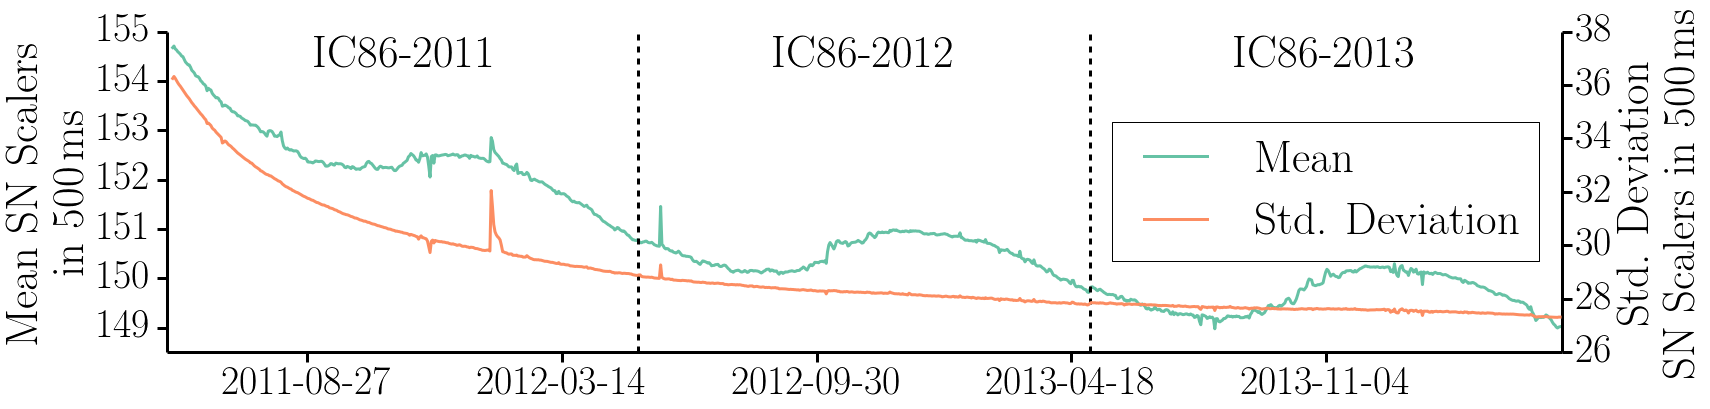
\includegraphics[width=0.95\textwidth]{graphics/dom/performance/darknoise/briedel1.png}
 \caption{Mean and variance of the supernova scaler distribution for the entire detector over the course of the first three
years of the completed IceCube \cite{briedel_phd}.}
 \label{fig:noise_over_time_briedel}
\end{figure}


The above mentioned 'freeze-in' related noise rate decay is even more clearly visible when we concentrate only on string deployed in the last drill season of IceCube, see Figure \ref{fig:noise_over_time_briedel_lastseasondepoyed}. Since the dark noise components are not correlated over several DOMs but are intrinsic to each individual DOM, the dark noise decay is not prominent in hits where neighboring DOMs are hit as well in a given time range (called HLC hits). Single DOM (or SLC) hits, on the other hand, represent exactly the decreasing noise rate behavior in the standard deviation of their corresponding SLC rate, as shown in Figure \ref{fig:slc_over_time_briedel}.

\begin{figure}[!h]
 \centering
 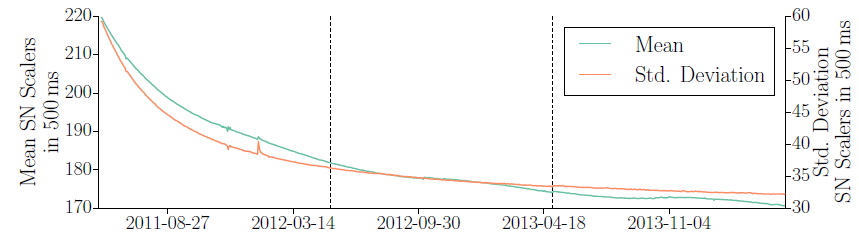
\includegraphics[width=0.95\textwidth]{graphics/dom/performance/darknoise/briedel4.png}
 \caption{Mean and standard deviation of the scaler rate of strings deployed in the last deployment season (austral summer of 2010/2011) \cite{briedel_phd}.}
 \label{fig:noise_over_time_briedel_lastseasondepoyed}
\end{figure}


\begin{figure}[!h]
 \centering
 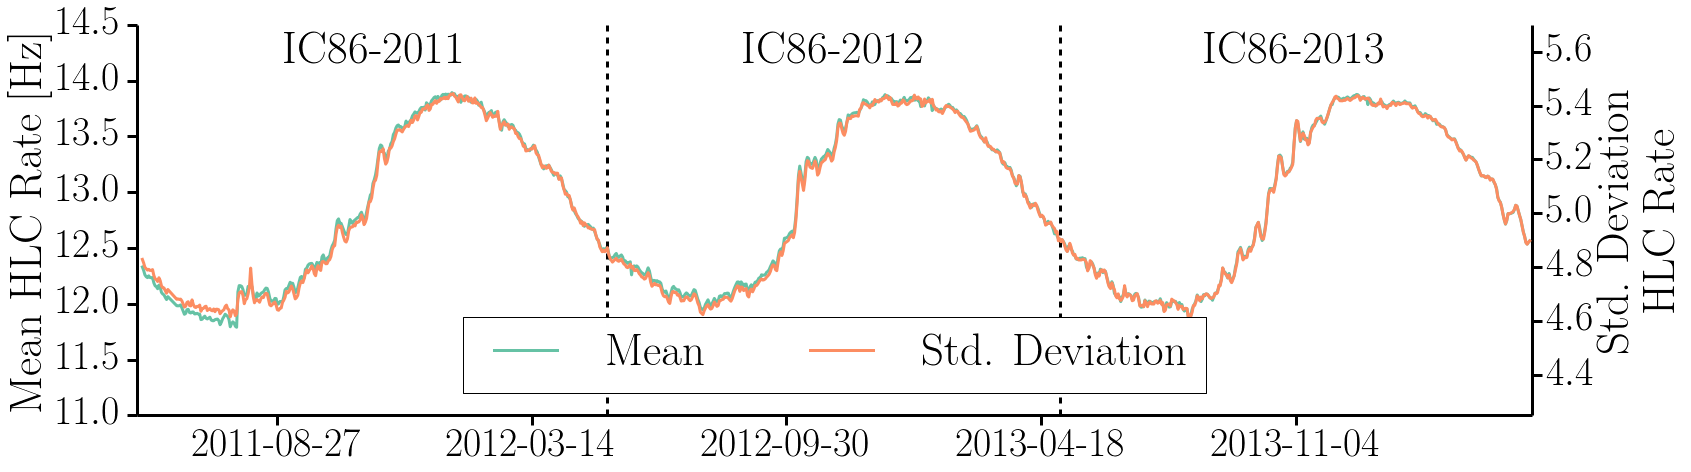
\includegraphics[width=0.95\textwidth]{graphics/dom/performance/darknoise/briedel2.png}
 \caption{Mean and standard deviation of the HLC rate distribution \cite{briedel_phd}.}
 \label{fig:hlc_over_time_briedel}
\end{figure}

\begin{figure}[!h]
 \centering
 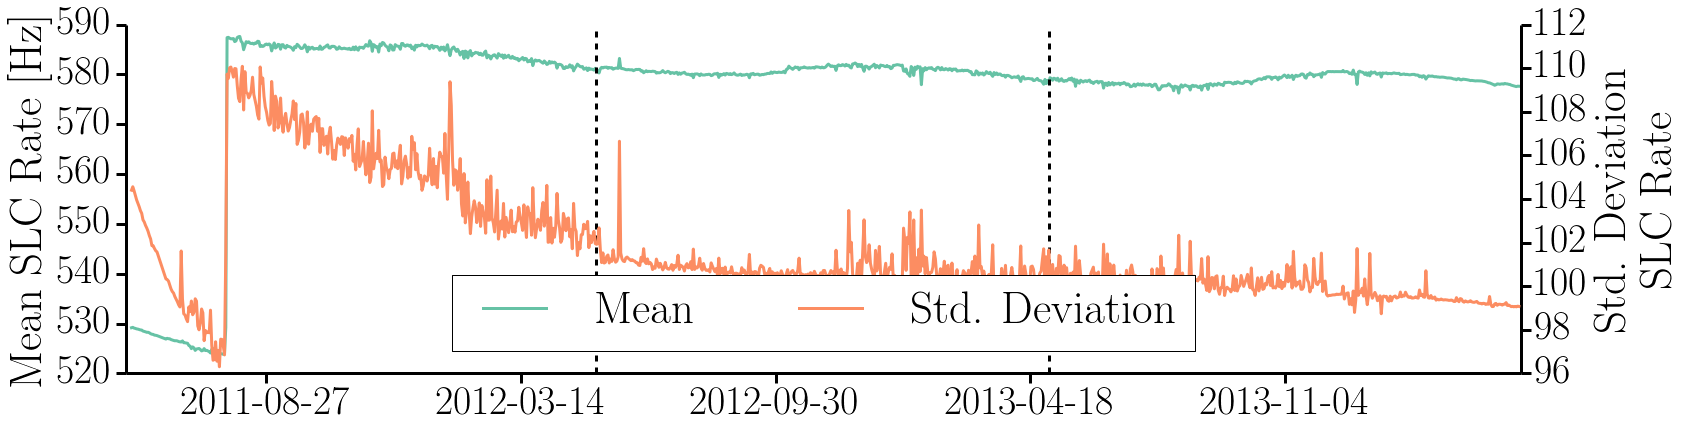
\includegraphics[width=0.95\textwidth]{graphics/dom/performance/darknoise/briedel3.png}
 \caption{Mean and standard deviation of the SLC rate distribution. The decay and jump in both quantities result from a change in the DOM deadtime by 10\%. \cite{briedel_phd}.}
 \label{fig:slc_over_time_briedel}
\end{figure}










%%%%%%%%%%%%%%%%%%%%%%%%%%
%
% following refs should be moved to top level
%
%%%%%%%%%%%%%%%%%%%%%%%%%%

%\begin{thebibliography}{9}

%IceCube energy reconstruction paper
%\bibitem{IC3:ereco} IceCube energy reconstruction paper

%IceCube standard candle reference
%\bibitem{IC3:SC} IceCube standard candle reference: Kiryluk et al proceedings ICRC 2007

%IceCube science description
%\bibitem{IC3:sci} IceCube Collaboration: J.~Ahrens {\it et al.}, Astropart. Phys. {\bf 20} (2004) 507

%IceCube original performance paper
%\bibitem{IC3:perf} IceCube Collaboration: A.~Achterberg  {\it et al.}, Astroparticle Physics {\bf 26} (2006) 155

%IceCube DOM-DAQ paper
%\bibitem{ref:domdaq}IceCube Collaboration: R.~Abbasi {\it et al.}, Nucl. Instr. and Methods in Phys. Res. A {\bf 601} (2009) 294

%IceCube PMT paper
%\bibitem{ref:pmt}IceCube Collaboration: R.~Abbasi {\it et al.}, Nucl. Instr. and Methods in Phys. Res. A {\bf 618} (2010) 139

%Characterization of large-area photomultipliers under low magnetic fields: 
%Design and performance of the magnetic shielding for the Double Chooz neutrino experiment
%\bibitem{ref:calvo} E.~Calvo {\it et al.}, Nucl. Instr. and Methods in Phys. Res. A {\bf 621} (2010) 222
%\end{thebibliography}
